% Chapter Template

\chapter{Demonstration and Debugging of sample scenarios} % Main chapter title

\label{Chapter5} % Change X to a consecutive number; for referencing this chapter elsewhere, use \ref{ChapterX}

\lhead{Chapter 5. \emph{Demonstration and debugging of sample scenarios}} % Change X to a consecutive number; this is for the header on each page - perhaps a shortened title

%----------------------------------------------------------------------------------------
%	SECTION 1
%----------------------------------------------------------------------------------------

This chapter is intended to demonstrate how a combination of relational data as well as the created
visualizations can help a network administrator to the state and understand the fault in the network.

We look at the following two problems here: The synchronous incast problem and the asynchronousincast problem.

\section{The Synchronous Incast Problem}

\subsection{Description}

This type of problem occurs in data centers in applications like MapReduce and DFS exhibiting fan-in traffic patterns.
This occurs when multiple hosts send data to a single host. In the case where the traffic from multiple hosts is
synchronized(common in scatter-gather architectures, Figure \ref{fig:Synch Incast}), it may lead to heavy congestion for a short duration (of the
order of microseconds\cite{microburst}) and lead to spikes in queuing delay even when none of the flows are individually anywhere near
the capacity of the link.

\begin{figure}[htbp]
	\centering
		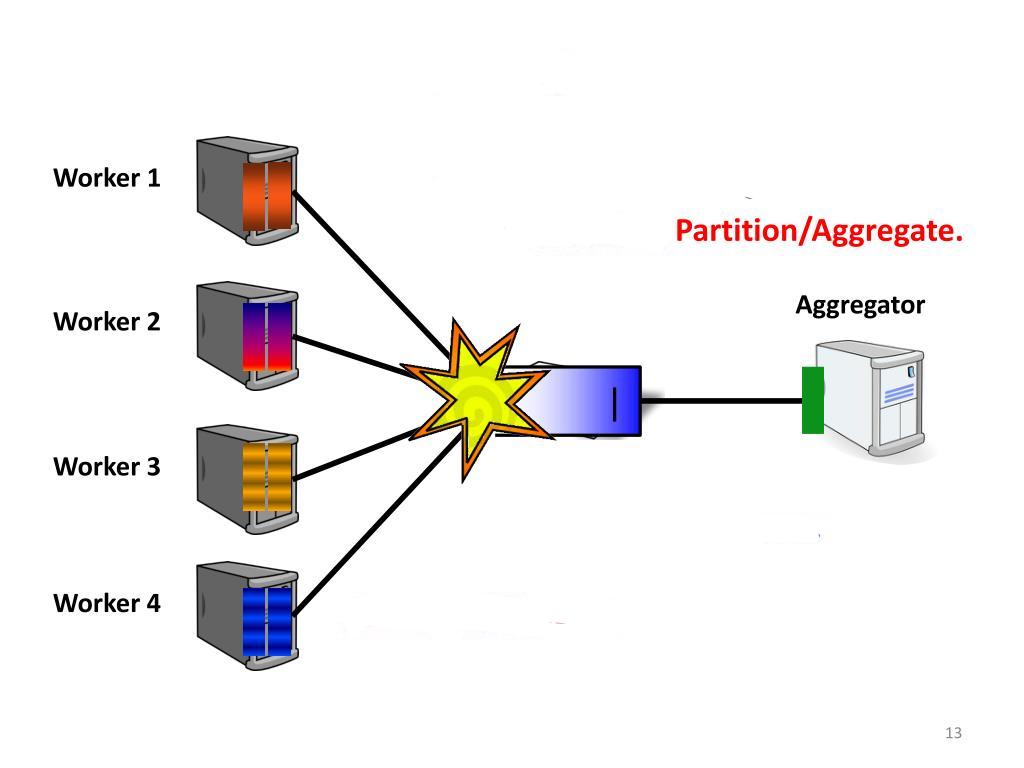
\includegraphics[width=0.65\columnwidth]{Figures/sync_incast.jpg}
		\rule{35em}{0.5pt}
	\caption[Synchronized Incast]{Synchronized Incast in Partition-Aggregate architecture}
	\label{fig:Synch Incast}
\end{figure}

\subsection{Configuration}
For creating a synchronized incast scenario in our topology, we generate traffic of 1 Gbps from hosts H1 to H6. The flow are routed
according to Figure \ref{fig:Synch Incast Topo} and get aggregated at switch 7.
\begin{figure}[htbp]
	\centering
		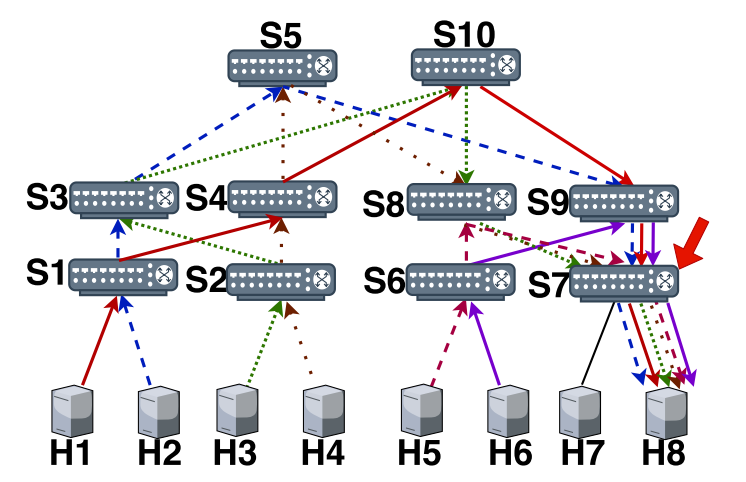
\includegraphics[width=0.65\columnwidth]{Figures/sync_incast_topo.png}
		\rule{35em}{0.5pt}
	\caption[Synchronized Incast Flows]{Synchronized Incast at switch 7 due to synchronized Fan-in traffic}
	\label{fig:Synch Incast Topo}
\end{figure}


\subsection{Diagnosis}
A synchronized microburst will often lead to multiple spikes occuring in a plot 
of the queue depth at the trigger switch. An algorithm for determining the width of
the peak queueDepth is described here.

\begin{algorithm}
	\caption{Estimate Width of Peak}
	\begin{algorithmic}[1]
		\REQUIRE indexOfPeak, records, peakDepth
		\STATE $leftThreshold \leftarrow 0.3, rightThreshold \leftarrow 0.5$
		\STATE $leftIndex = indexOfPeak - 1$
		\STATE $rightIndex = indexOfPeak + 1$
		% \WHILE{$leftIndex \geq 0$}
		
		\WHILE{$records[leftIndex].depth \geq leftThreshold \times peakDepth$}
		\STATE $leftIndex = leftIndex - 1$
		\ENDWHILE

		\WHILE{$records[rightIndex].depth \geq rightThreshold \times peakDepth$}
		\STATE $rightIndex = rightIndex + 1$
		\ENDWHILE

		\STATE $width = records[rightIndex].timeOut - records[leftIndex].timeIn$
		% \ENDWHILE
		% }
	\end{algorithmic}
\end{algorithm}

Once the peak is estimated, we look at the distribution of packets that came into the queue during the peak
as well as the packets that were present in the queue at the start of the peak.
We use Jain's Fairness Index (Appendix \ref{AppendixA}) to estimate fairness of distribution of packets according to source IP.
If the Jain's Fairness Index turns out to be greater than a predetermined threshold of 0.7, then it is classified as a case of 
Synchronized Incast due to the observation that in a synchronized incast, the distribution of packets is mostly fair.
\subsection{Results and Illustrations}
The above heuristic was applied in 5 different scenarios of synchronized incast of varied transmission rates.
The resultant values of Fairness Index calculated are given in table \ref{tab:J_Index_Sync}
\begin{table}[h]
\begin{center}
\begin{tabular}{ |p{3cm}|p{3cm}|  }
	\hline
	\multicolumn{2}{|c|}{Jain's Index} \\
	\hline
	Scenario & Value \\
	\hline
	1 & 0.957 \\
	2 & 0.980 \\
	3 & 0.890 \\
	4 & 0.780 \\
	5 & 0.975 \\
	\hline
   \end{tabular}
\end{center}

\caption{Jain's Index Values for different scenarios of Synchronous Incast}
% Help
\label{tab:J_Index_Sync}
\end{table}
The operator first looks at the readings of Jain's Index (Fig. \ref{fig:jind_sync} which point him towards the fact that it is a possible
case of synchronized incast.
Then he looks at the birds eye view of the network and seens that all flows seem to converge at the trigger switch at the same time (Fig. \ref{fig:genview_sync}).
Further, to help the network operator visualize the scenario, plots of queue depth at the
trigger switch are plotted, along with packet distribution in the estimated peak, as shown in figures \ref{fig:queue_depth_sync}
and \ref{fig:distribution_sync}.
The operator then looks at the plot of ingress throughput and concludes that all the flows entered the switch
at roughly the same time, and there is a certain periodicity in their arrival, as shown in Fig. \ref{fig:ing_sync}
These hints are enough to suggest to him that the problem is of a synchronous incast.

\begin{figure}[htbp]
	\centering
		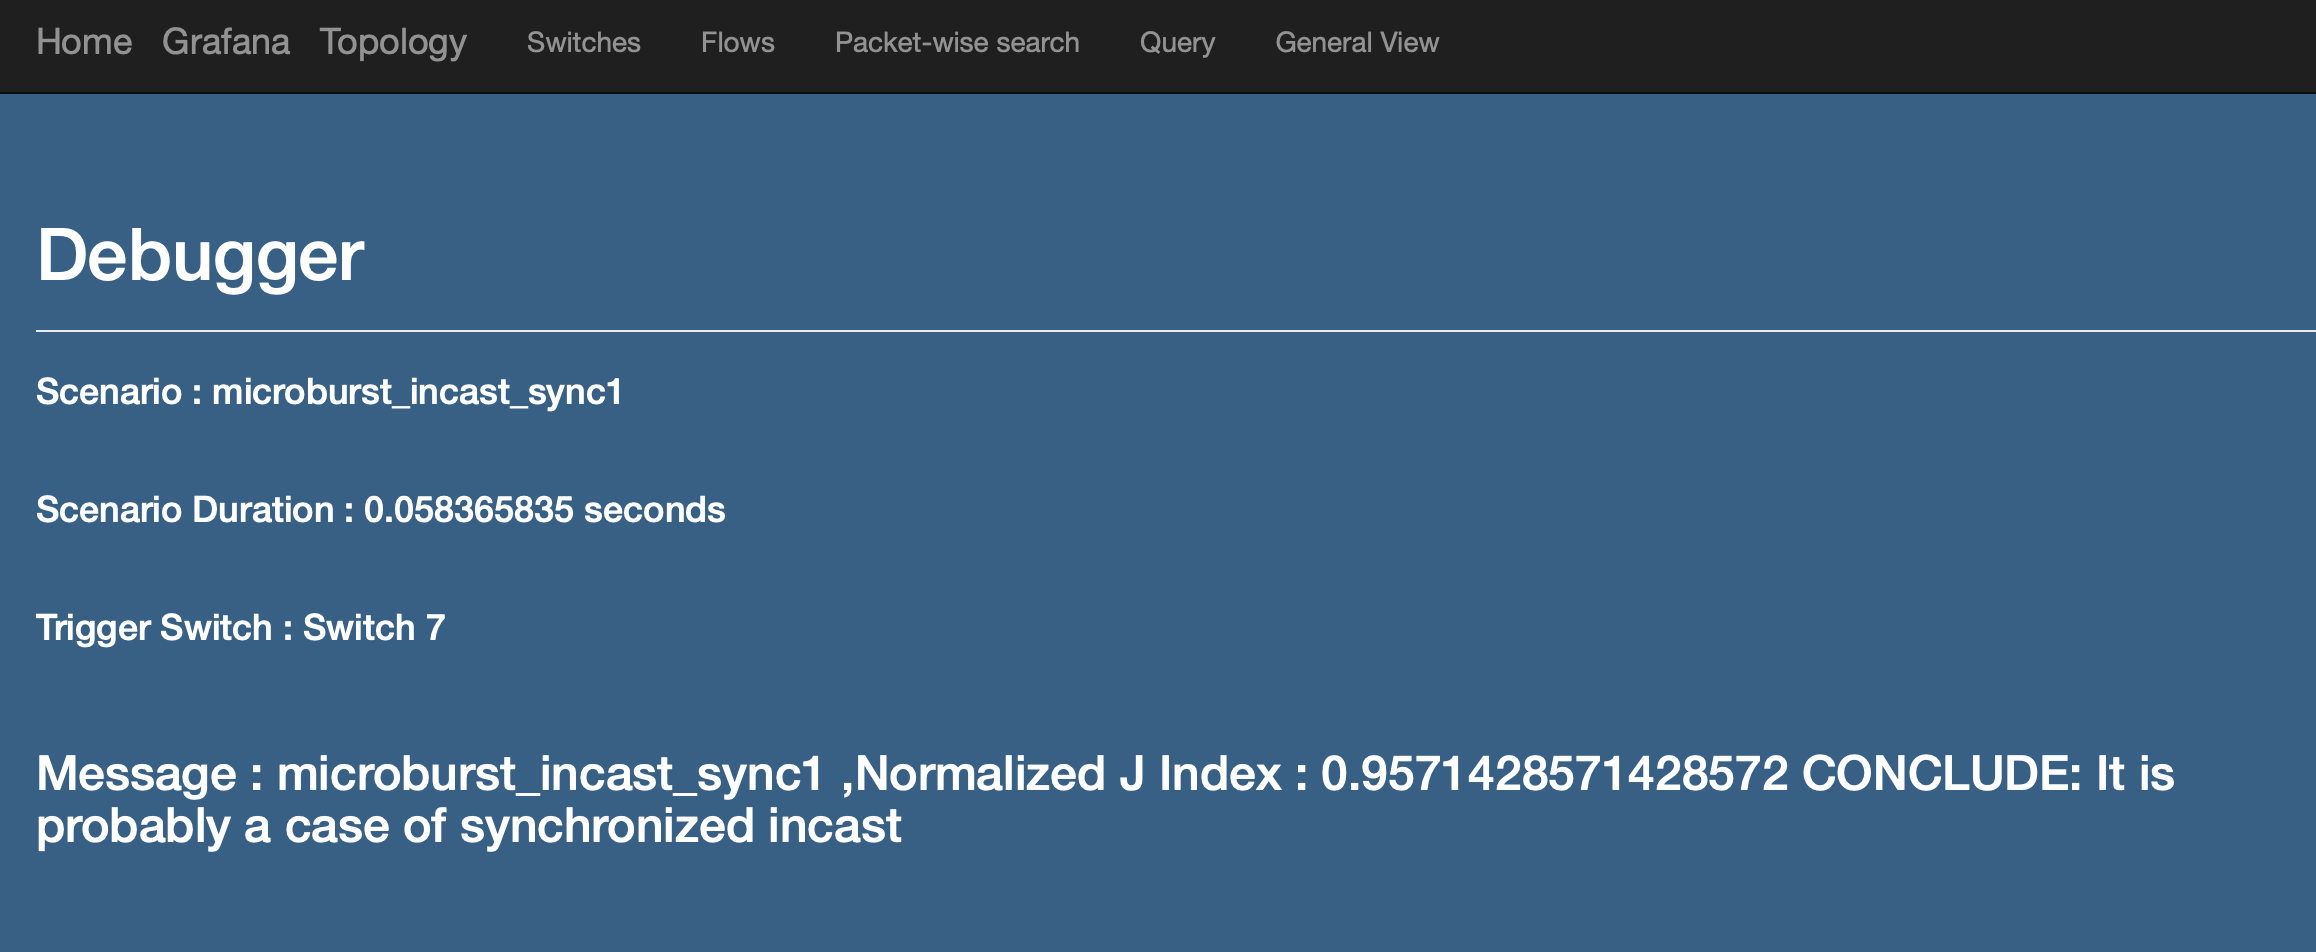
\includegraphics[width=1.0\columnwidth]{Figures/jindex_sync.png}
		\rule{35em}{0.5pt}
	\caption[Debugger Home Page, Synchronous Incast]{J Index calculated and presented to administrator}
	\label{fig:jind_sync}
\end{figure}

\begin{figure}[htbp]
	\centering
		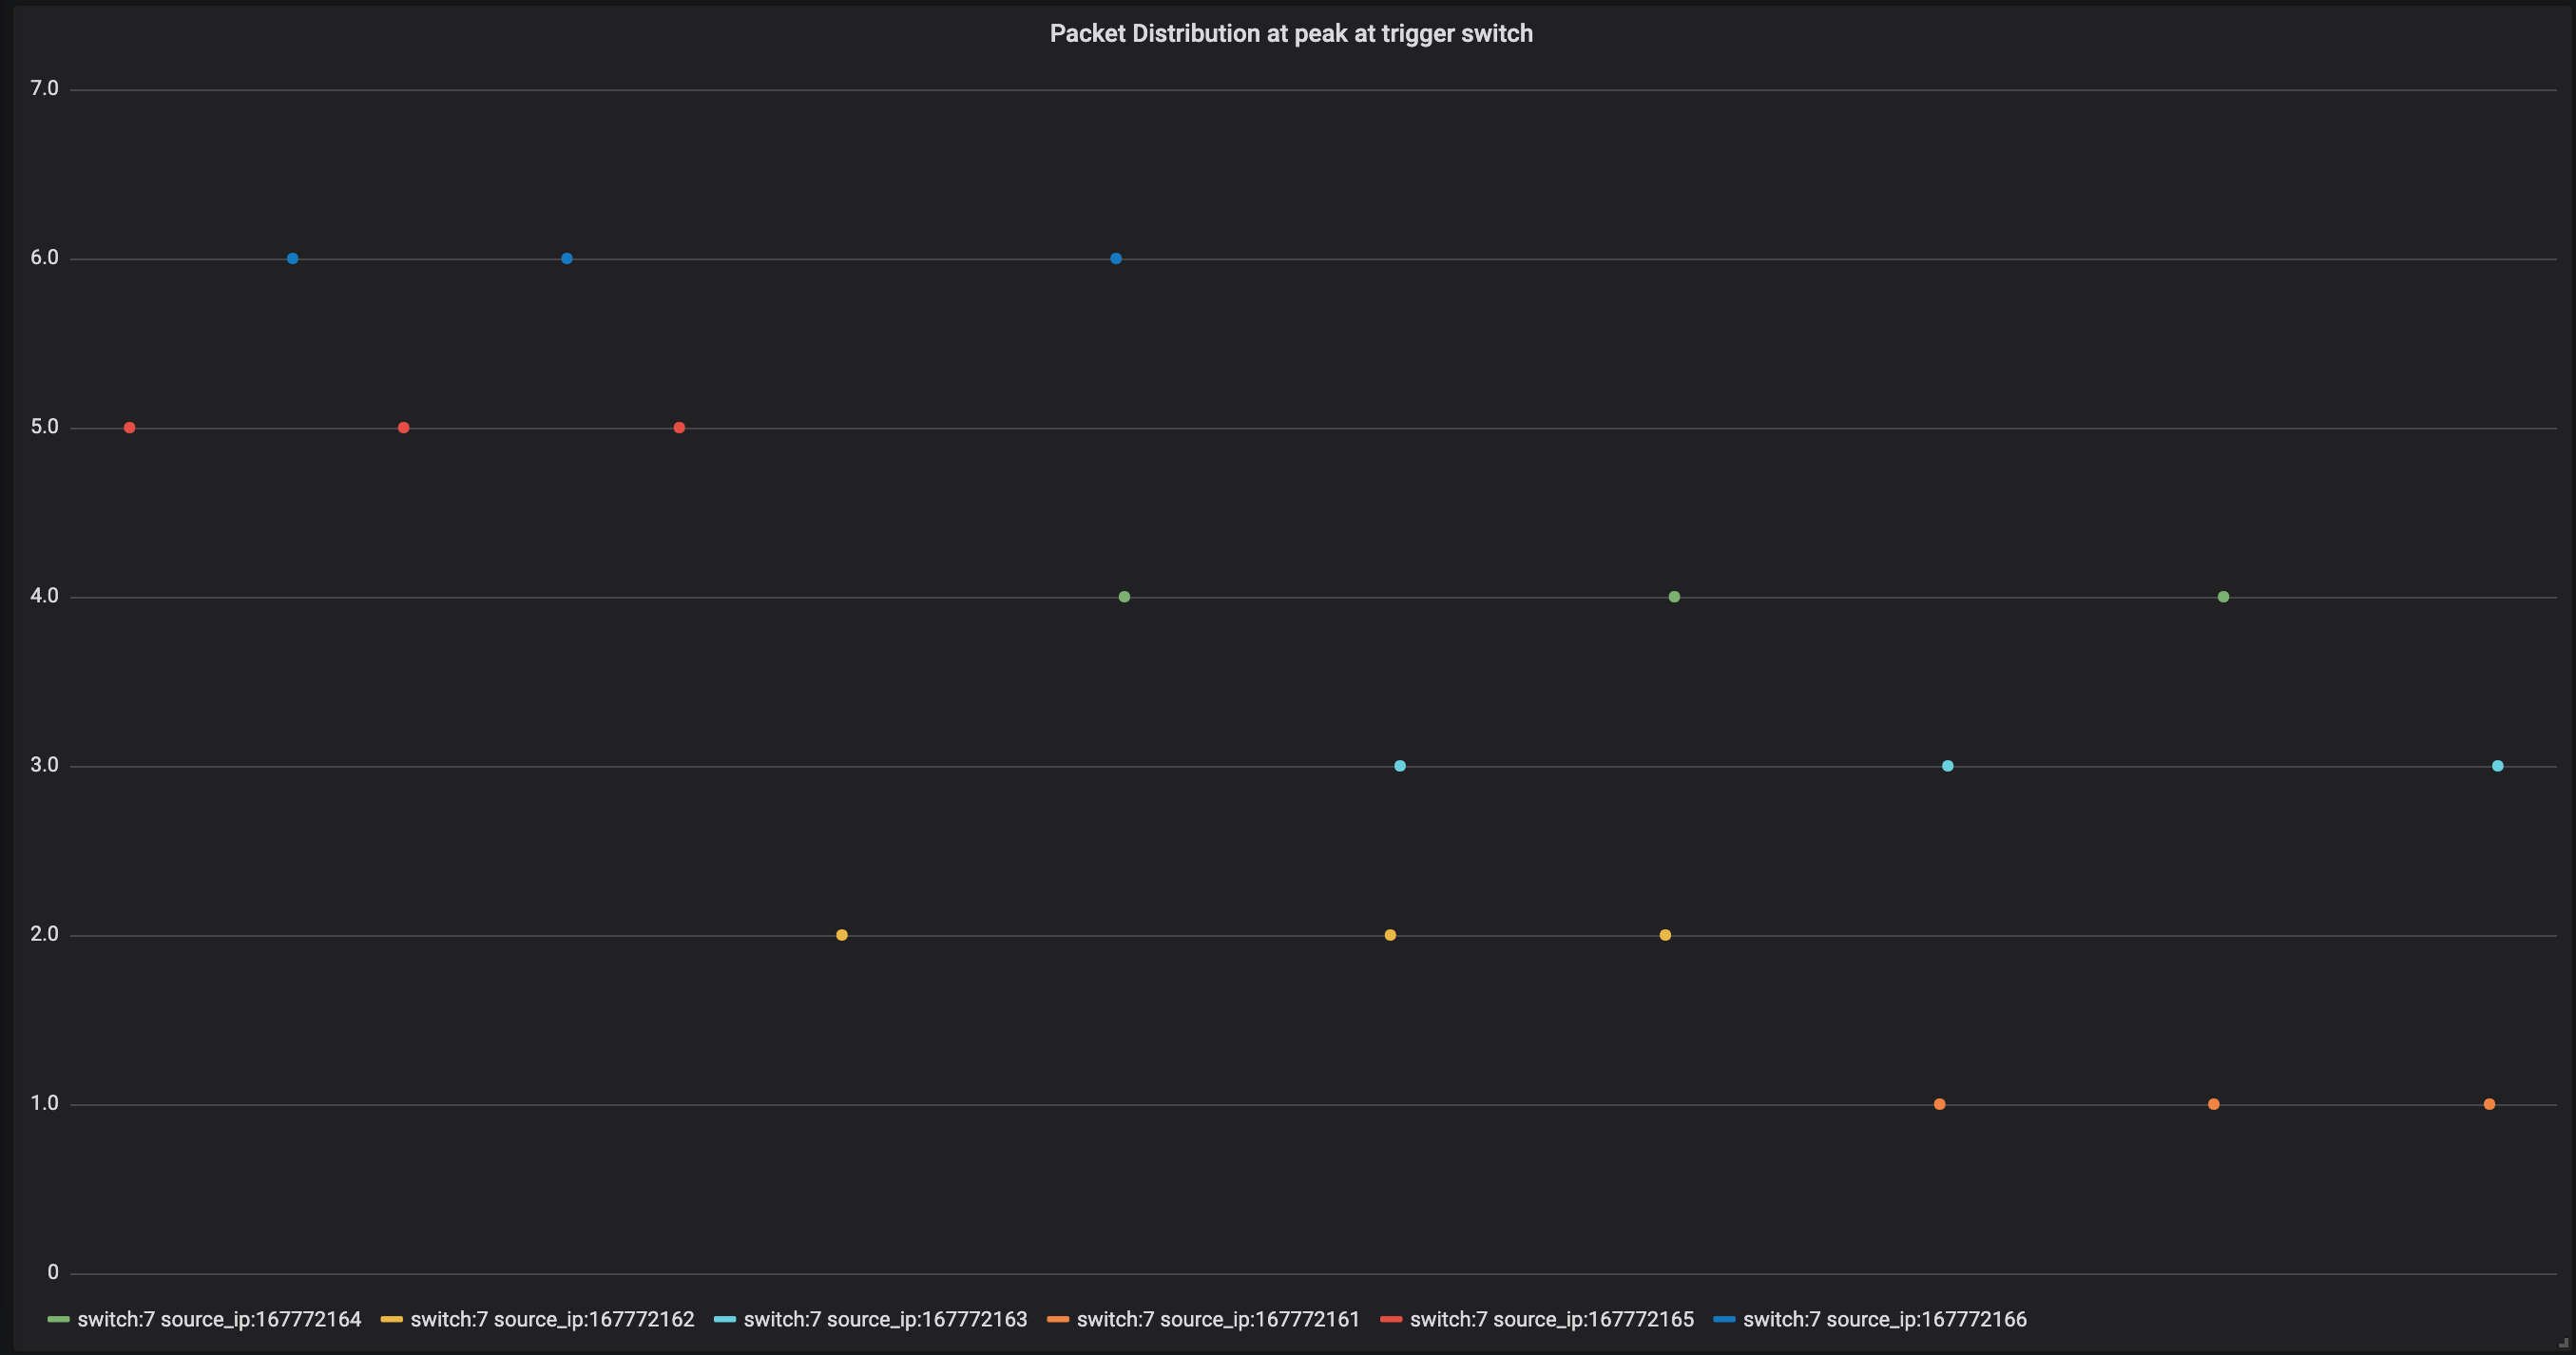
\includegraphics[width=1.0\columnwidth]{Figures/distribution_sync.png}
		\rule{35em}{0.5pt}
	\caption[Packet Distribution at Trigger Switch, Sync Incast]{Packet Distribution at Trigger Switch, Sync Incast. Note the highly even distribution.}
	\label{fig:distribution_sync}
\end{figure}

\begin{figure}[htbp]
	\centering
		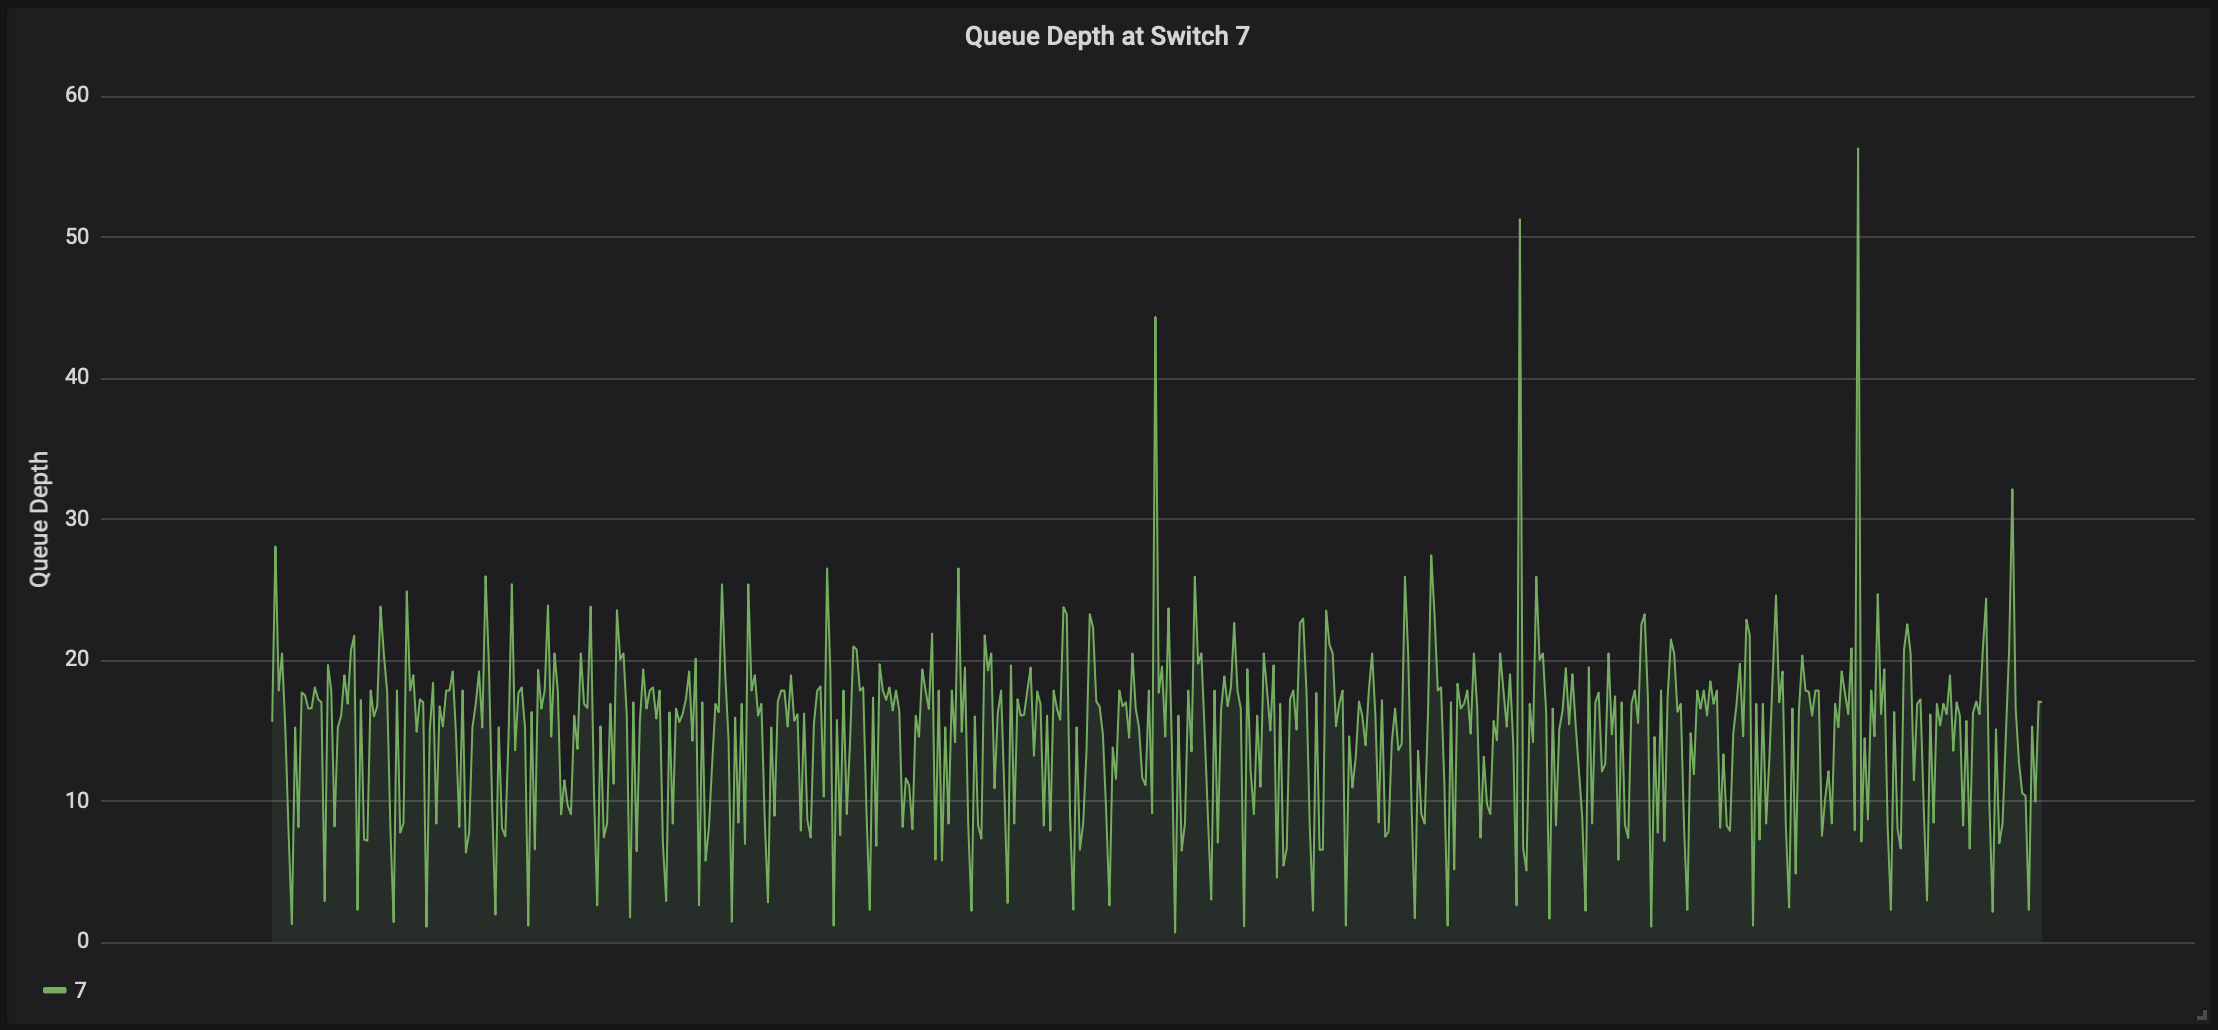
\includegraphics[width=1.0\columnwidth]{Figures/queue_depth_sync.png}
		\rule{35em}{0.5pt}
	\caption[Queue Depth at Trigger Switch, Sync Incast]{Queue Depth at Trigger Switch, Sync Incast}
	\label{fig:queue_depth_sync}
\end{figure}

\begin{figure}[htbp]
	\centering
		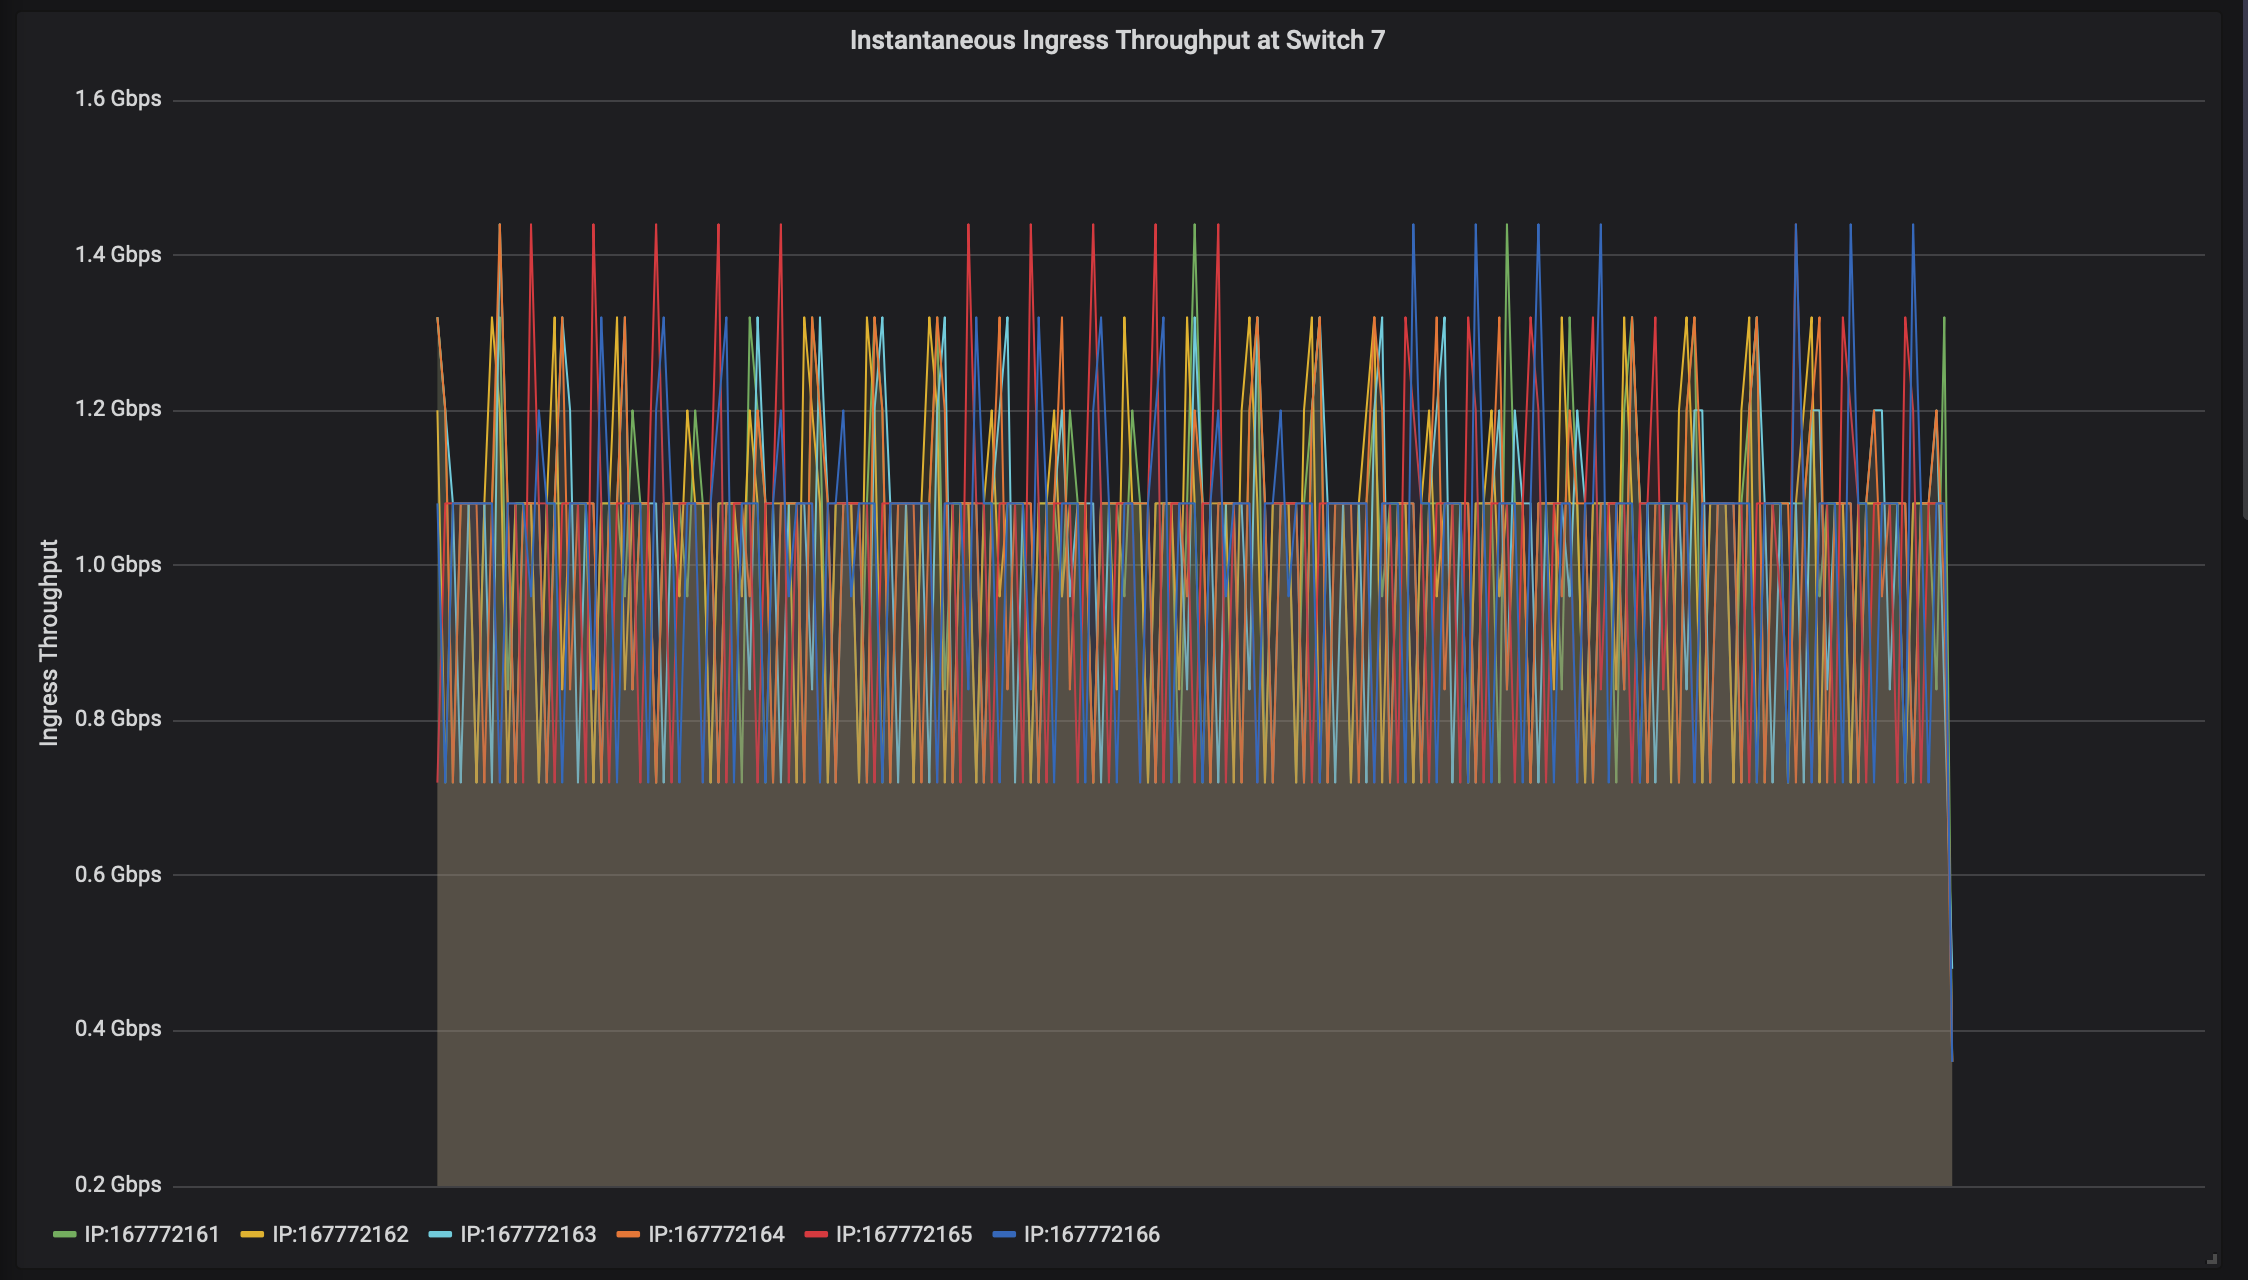
\includegraphics[width=1.0\columnwidth]{Figures/ingress_sync.png}
		\rule{35em}{0.5pt}
	\caption[Ingress Throughput for Synchronous Incast]{Ingress throughput for synchronous incast.}
	\label{fig:ing_sync}
\end{figure}

\begin{figure}[htbp]
	\centering
		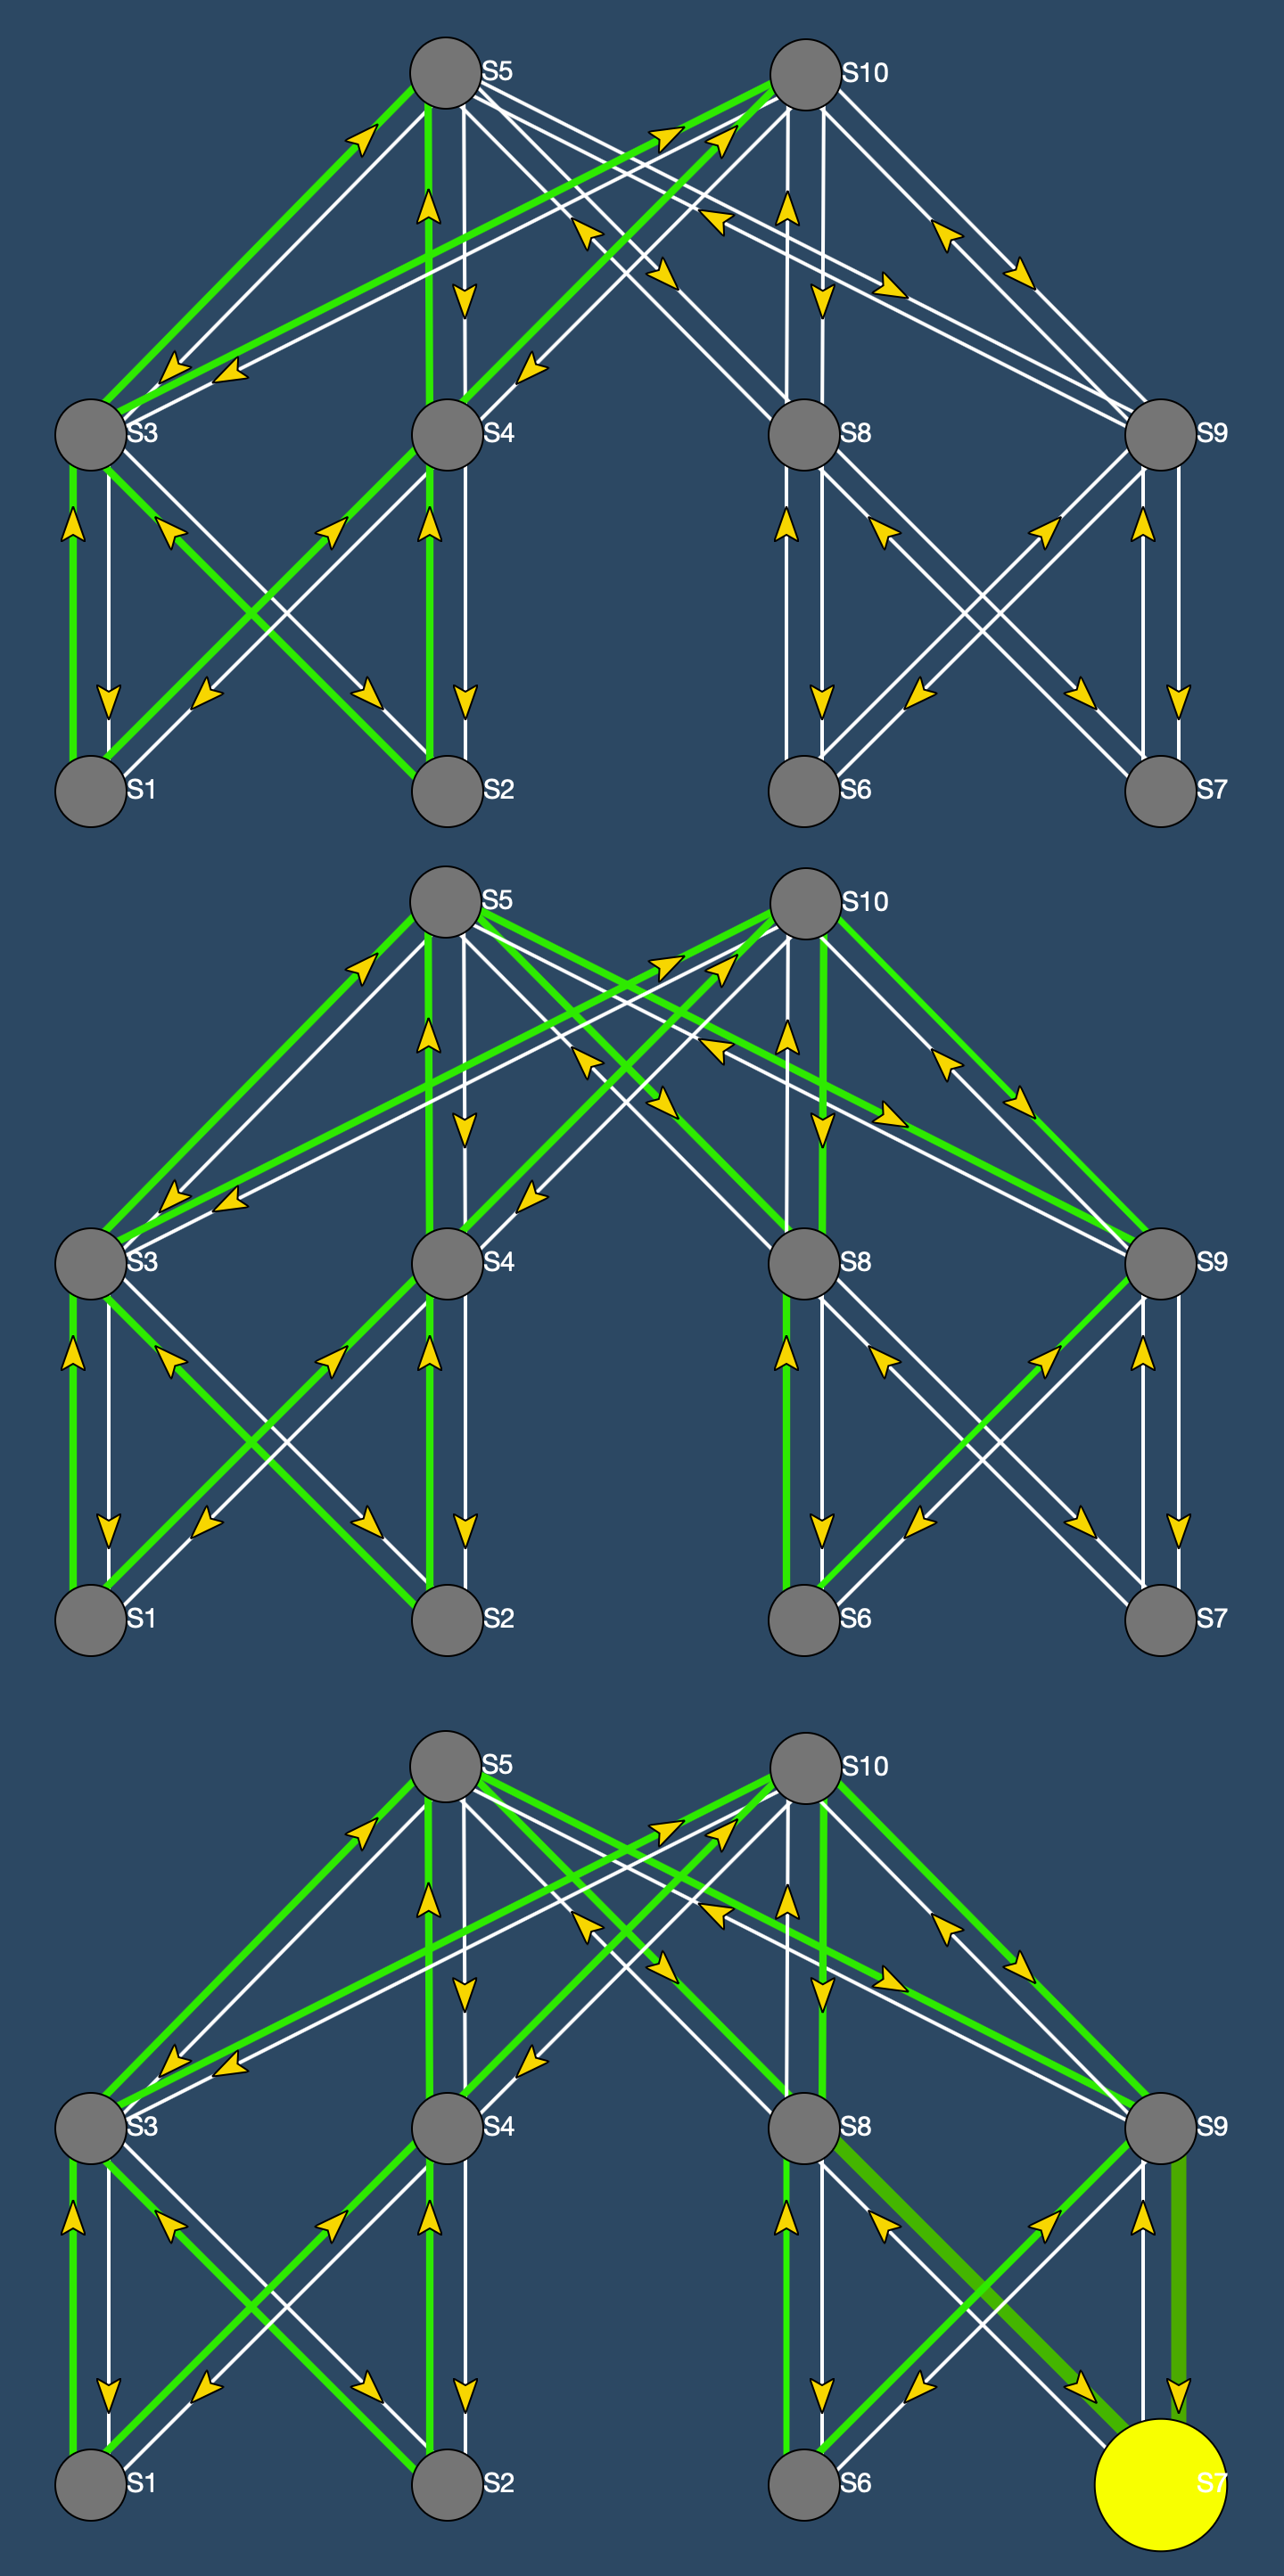
\includegraphics[width=20cm,height=25cm,keepaspectratio]{Figures/genview_sync.png}
		\rule{35em}{0.5pt}
	\caption[Birds eye view, Synchronous Incast]{Birds eye view of network at chronological points in time.}
	\label{fig:genview_sync}
\end{figure}

\section{Asynchronous Incast problem and Heavy Hitters}
\subsection{Description}
The Asynchronous Incast problem simply means a scenario where the queue depth increases over a period of microbursts
in the lack of any visible synchronization pattern. Often in these cases, we have the presence of a heavy hitter flow\cite{HH}
(A flow which consumes a substantial amount of bandwidth that violates fairness) which causes congestion and overflowing
of buffers in switch.
\subsection{Configuration}
For creating an asynchronous incast scenario in our topology, we generate traffic of 1 Gbps from H1, H3, H4 and 6 Gbps from H6. The flow are routed
according to Figure \ref{fig:Synch Incast Topo} and get aggregated at switch 7.
\subsection{Diagnosis}
In cases of asynchronous incast with heavy hitters, we will see a single large peak in the plot of queue depth and usually a very
skewed distribution in the peak. The heuristic used here is similar to the one in synchronous incast except if the Jain's 
Fairness Index is less that 0.45, then it is classified as an asynchronous incast problem.
\subsection{Results and Illustrations}

The above heuristic was applied in 5 different scenarios of aynchronous incast of varied transmission rates.
The resultant values of Fairness Index calculated are given in table \ref{tab:J_Index_Async}.
\begin{table}[h]
	\begin{center}
	\begin{tabular}{ |p{3cm}|p{3cm}|  }
		\hline
		\multicolumn{2}{|c|}{Jain's Index} \\
		\hline
		Scenario & Value \\
		\hline
		1 & 0.469 \\
		2 & 0.362 \\
		3 & 0.383 \\
		4 & 0.418 \\
		5 & 0.403 \\
		\hline
	   \end{tabular}
	\end{center}
	
	\caption{Jain's Index Values for different scenarios of Asynchronous Incast}
	% Help
	\label{tab:J_Index_Async}
	\end{table}

	The operator first looks at the readings of Jain's Index (Fig. \ref{fig:jind_async} which point him towards the fact that it is a possible
	case of asynchronized incast.
	Then he looks at the birds eye view of the network and seens that there is an interval of time when the links along a path fill up
	with traffic. (Fig. \ref{fig:genview_async}).
	Further, to help the network operator visualize the scenario, plots of ingress throughput and compositon of queue depth at 
	trigger switch are plotted, along with packet distribution in the estimated peak, as shown in figures \ref{fig:ing_throughput_async}, \ref{fig:queue_comp_async}
	and \ref{fig:distribution_async}
	Looking at the plot of ingress throughput, the operator sees that there is one heavyhitter flow with a rough throughputof 8 Gbps existing in the network.
	He also looks at the composition of the queue depth to see that a large number of packets at the peak are of the green flow (the heavy hitter).

	These hints suggest a case of asynchronous incast.

	\begin{figure}[htbp]
		\centering
			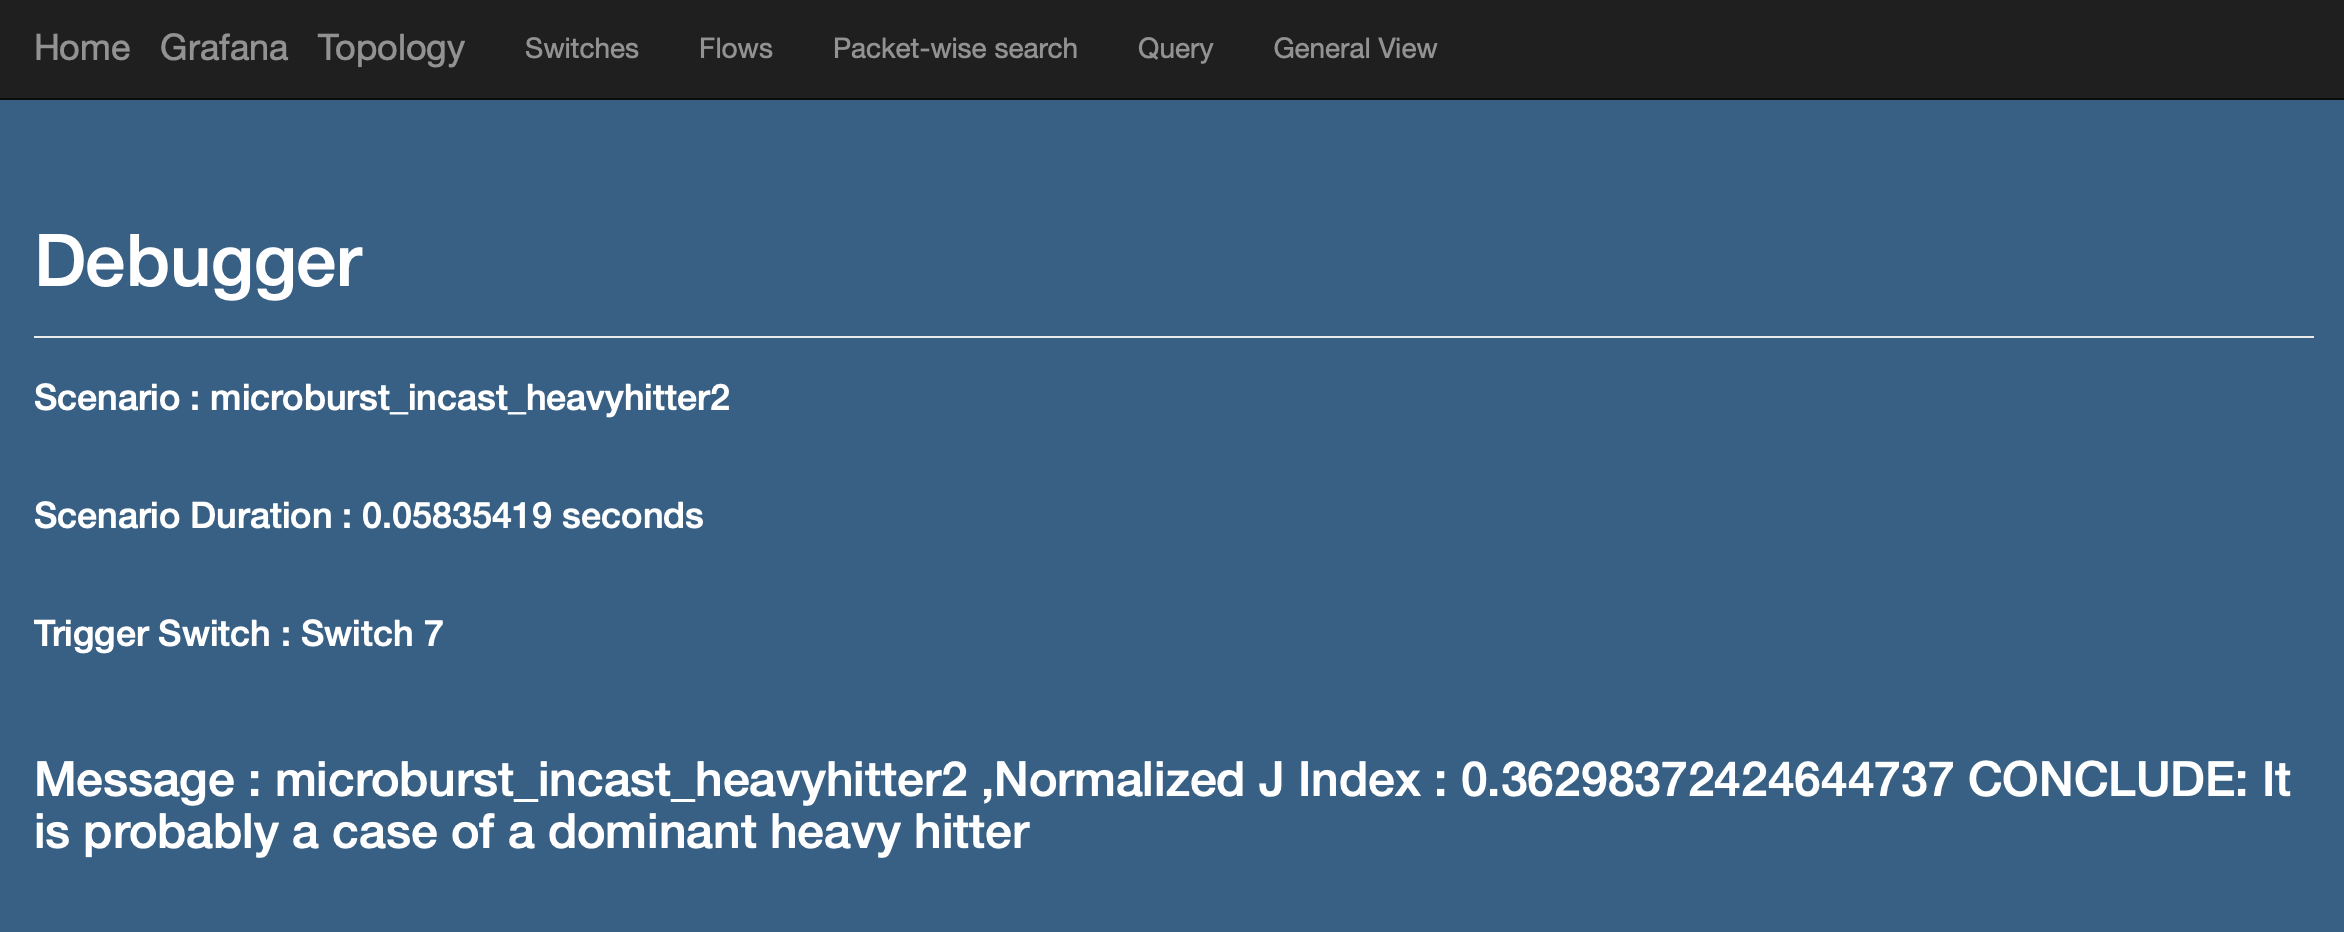
\includegraphics[width=1.0\columnwidth]{Figures/jindex_async.png}
			\rule{35em}{0.5pt}
		\caption[Debugger Home Page, Asynchronous Incast]{J Index calculated and presented to administrator}
		\label{fig:jind_async}
	\end{figure}

\begin{figure}[htbp]
	\centering
		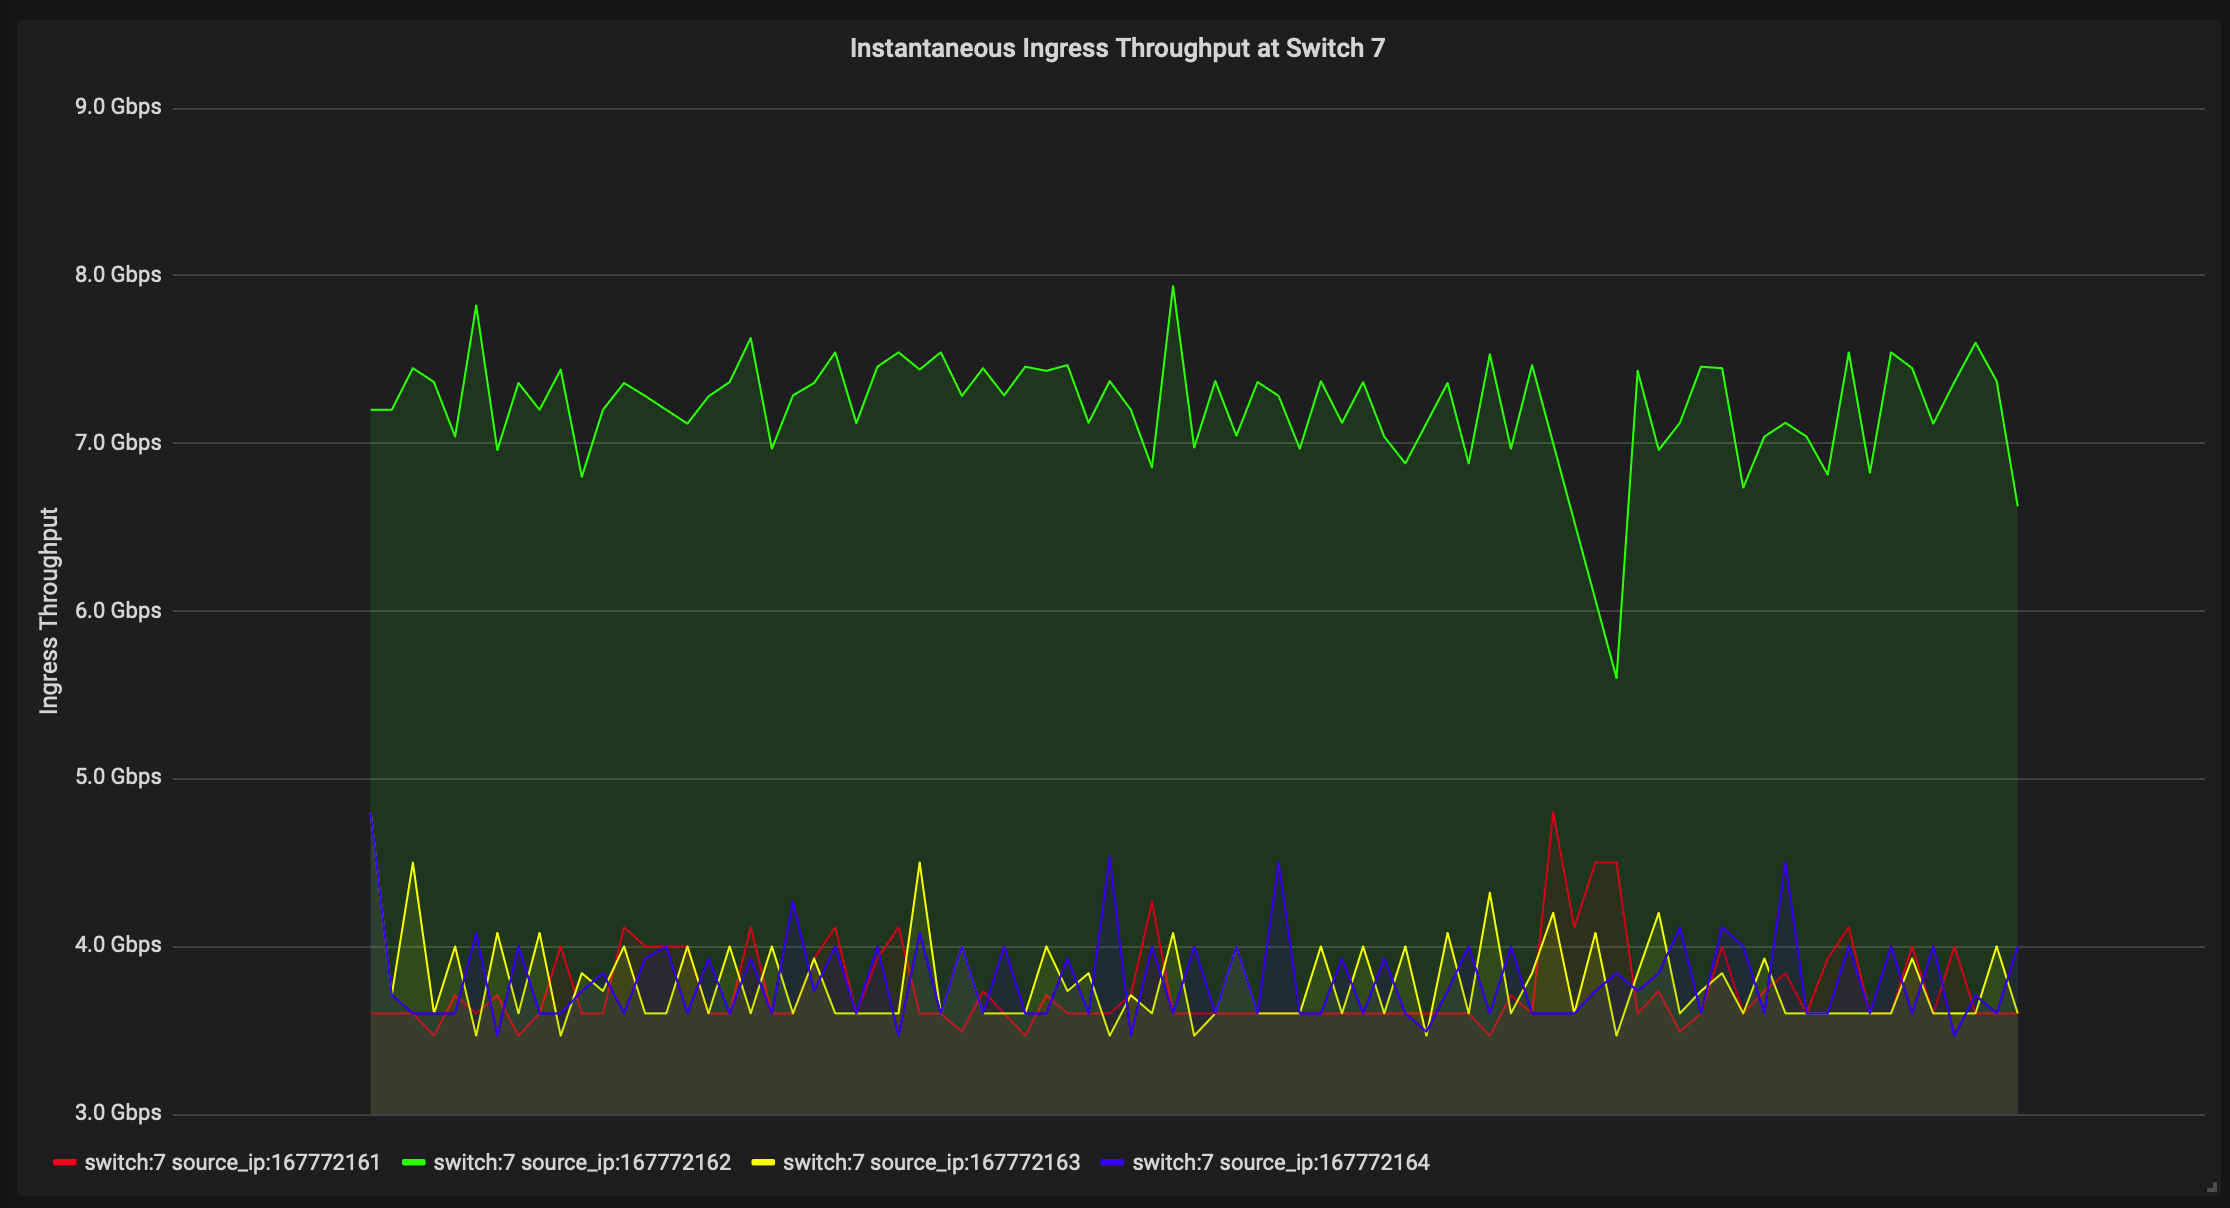
\includegraphics[width=1.0\columnwidth]{Figures/ing_thpt_async.png}
		\rule{35em}{0.5pt}
	\caption[Ingress Throughput Asynchronous Incast]{Ingress throughput for asynchronous incast}
	\label{fig:ing_throughput_async}
\end{figure}

\begin{figure}[htbp]
	\centering
		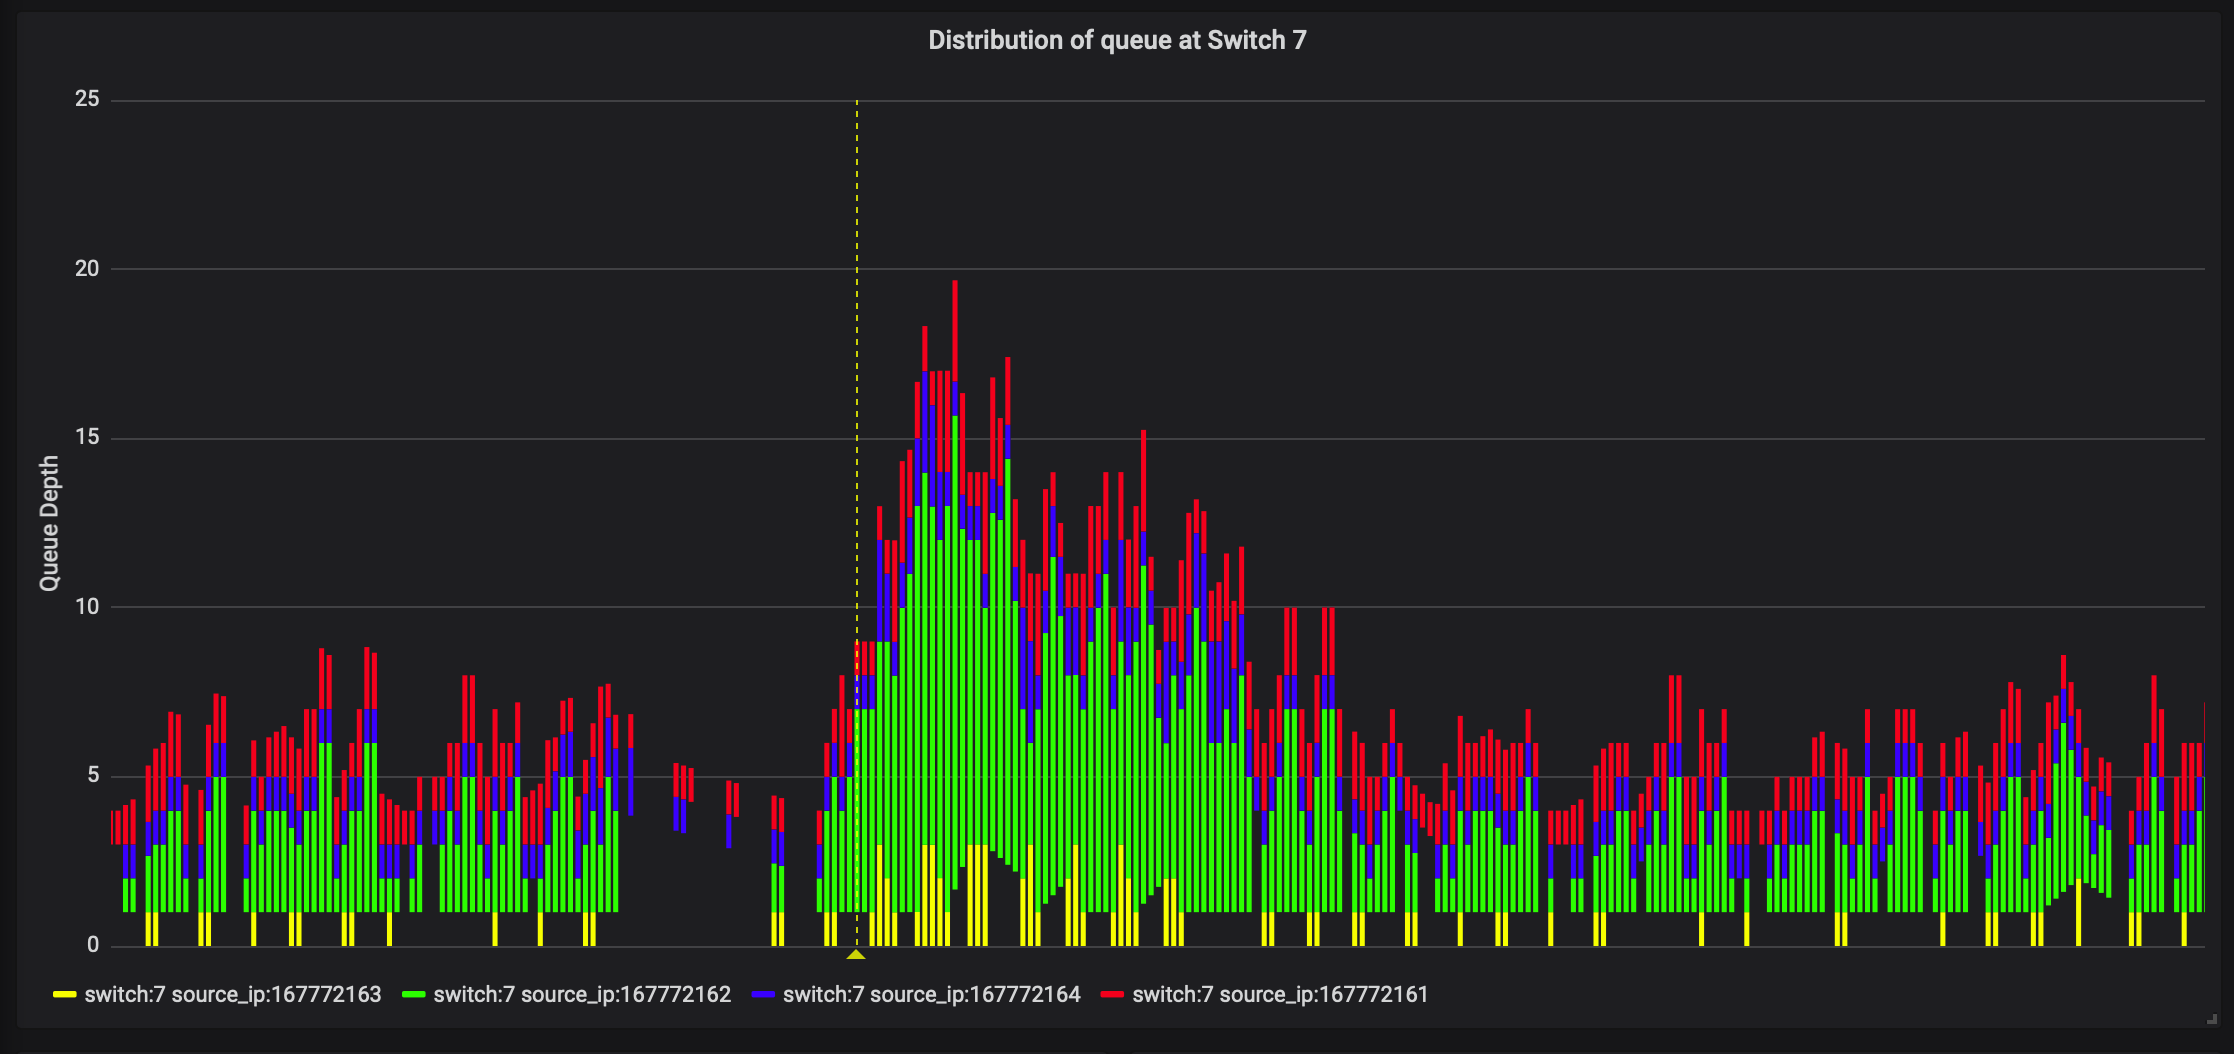
\includegraphics[width=1.0\columnwidth]{Figures/queue_comp_async.png}
		\rule{35em}{0.5pt}
	\caption[Queue Composition at Trigger Switch, Async Incast]{Queue Composition at Trigger Switch, Async Incast}
	\label{fig:queue_comp_async}
\end{figure}
\begin{figure}[htbp]
	\centering
		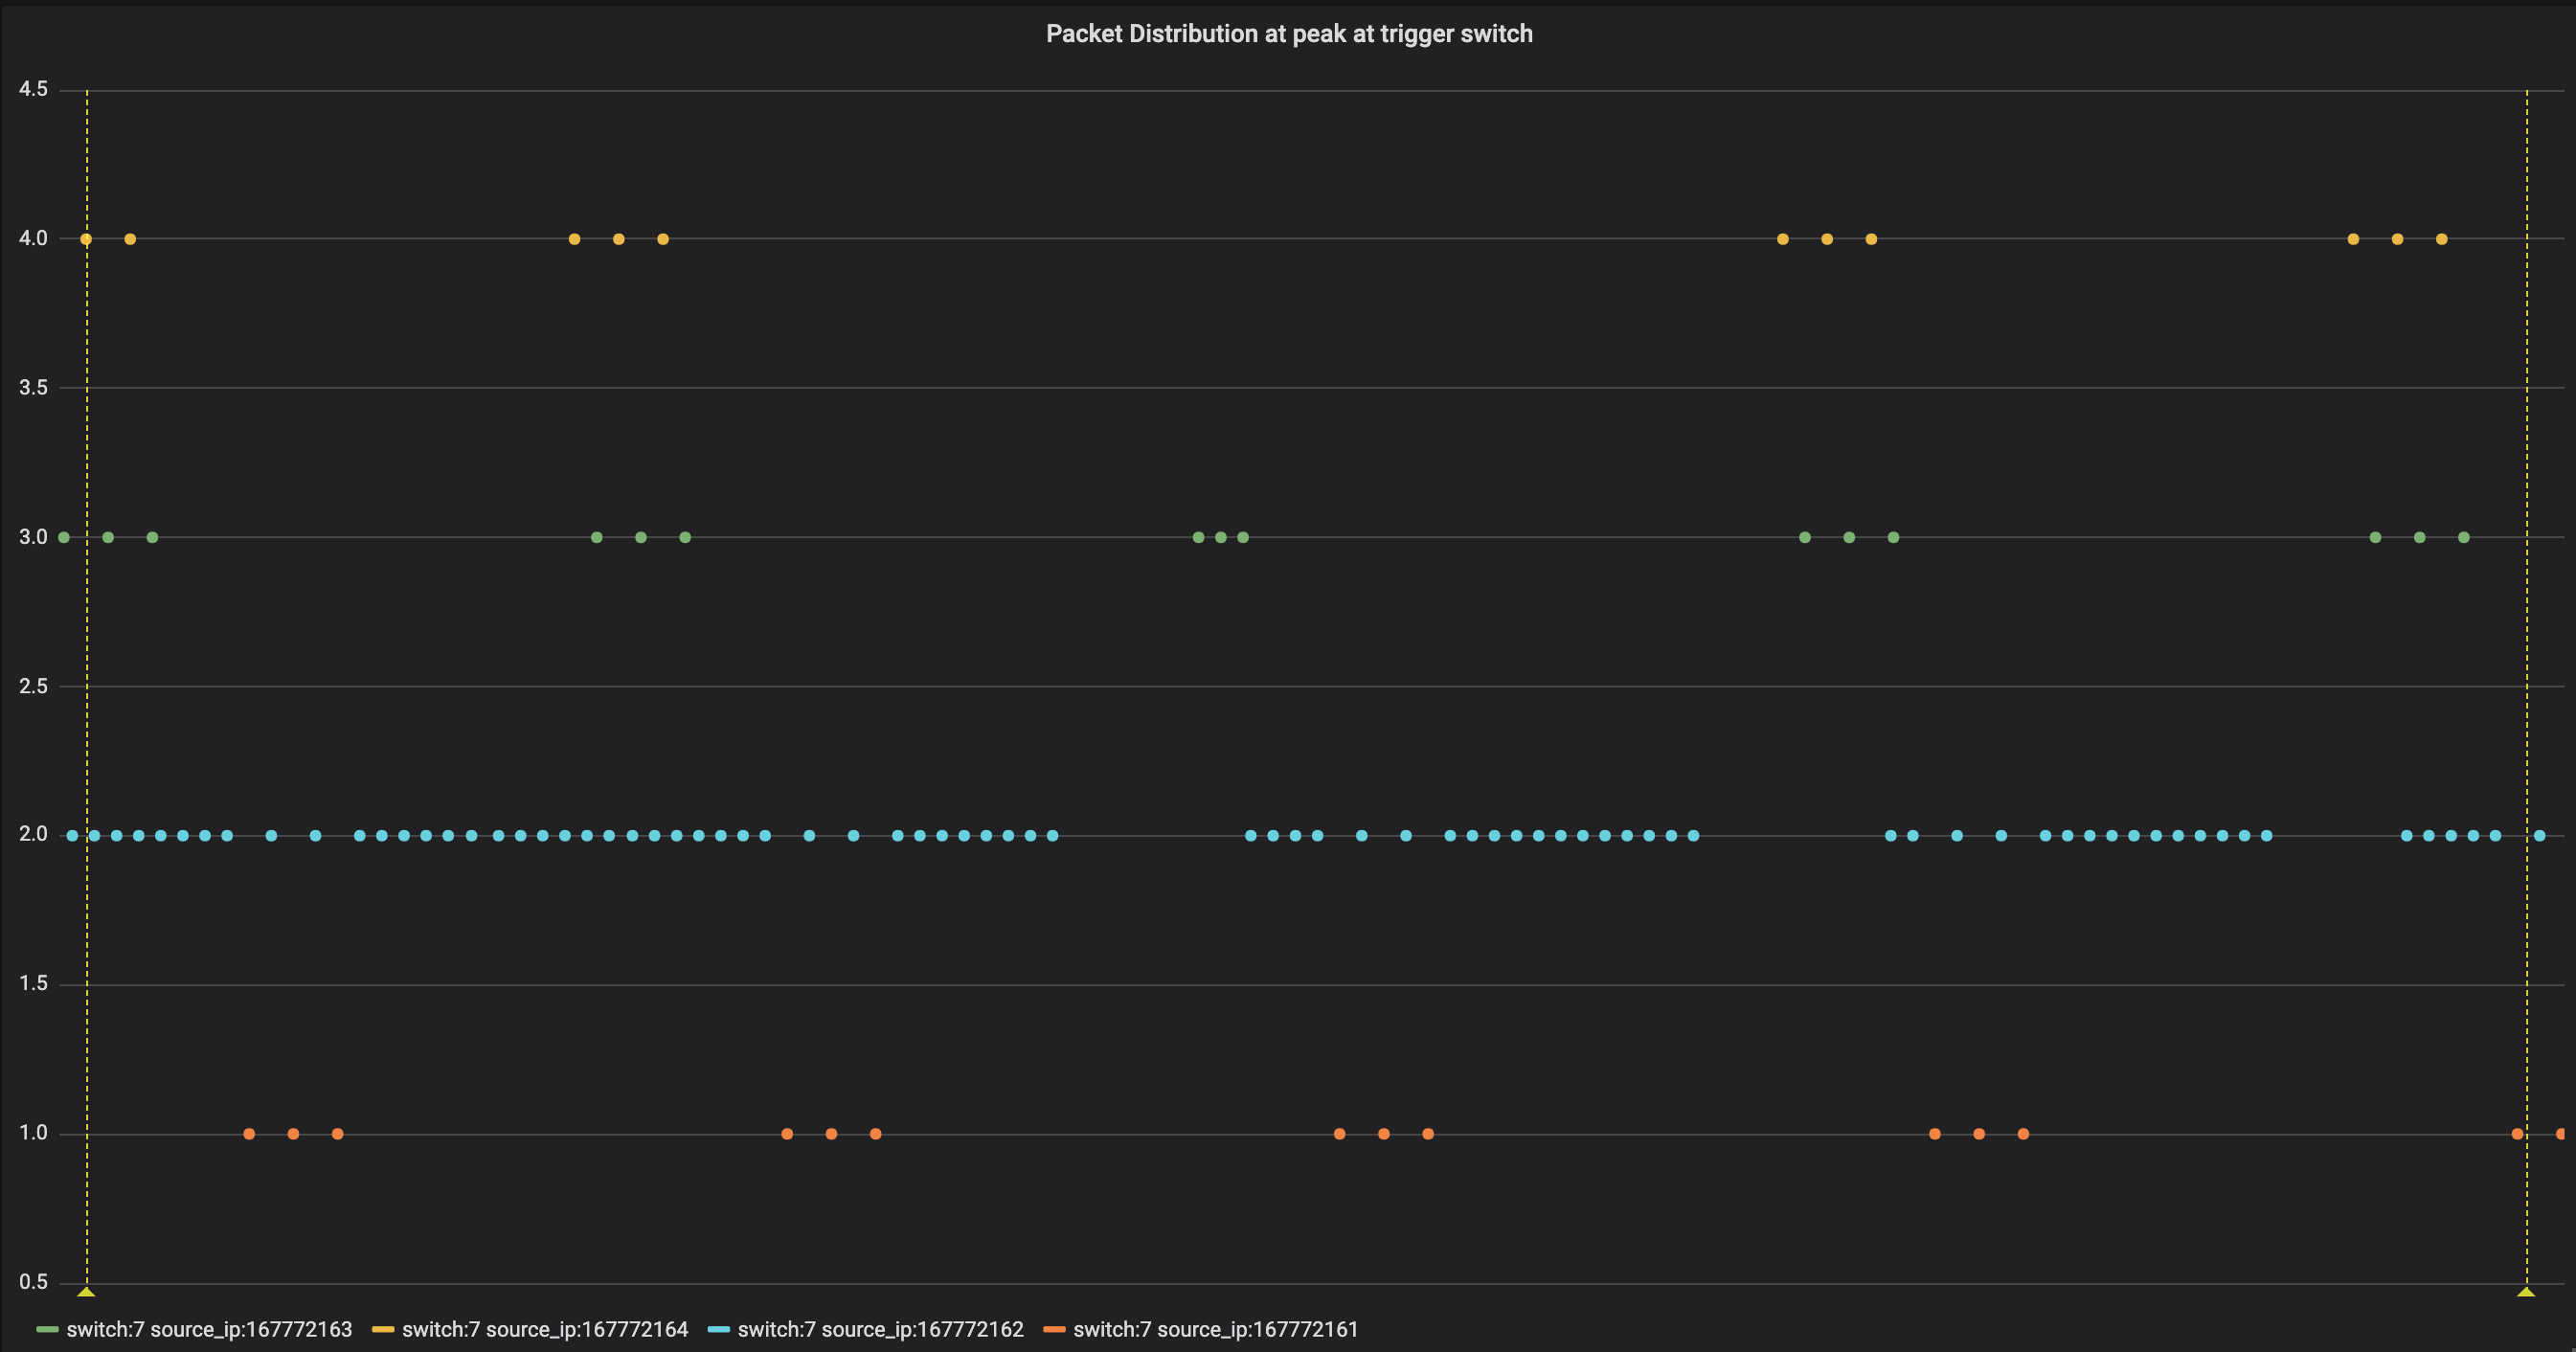
\includegraphics[width=1.0\columnwidth]{Figures/distribution_async.png}
		\rule{35em}{0.5pt}
	\caption[Packet Distribution at Trigger Switch, Async Incast]{Packet Distribution at Trigger Switch, Async Incast. Note the highly skewed distribution.}
	\label{fig:distribution_async}
\end{figure}

\begin{figure}[htbp]
	\centering
		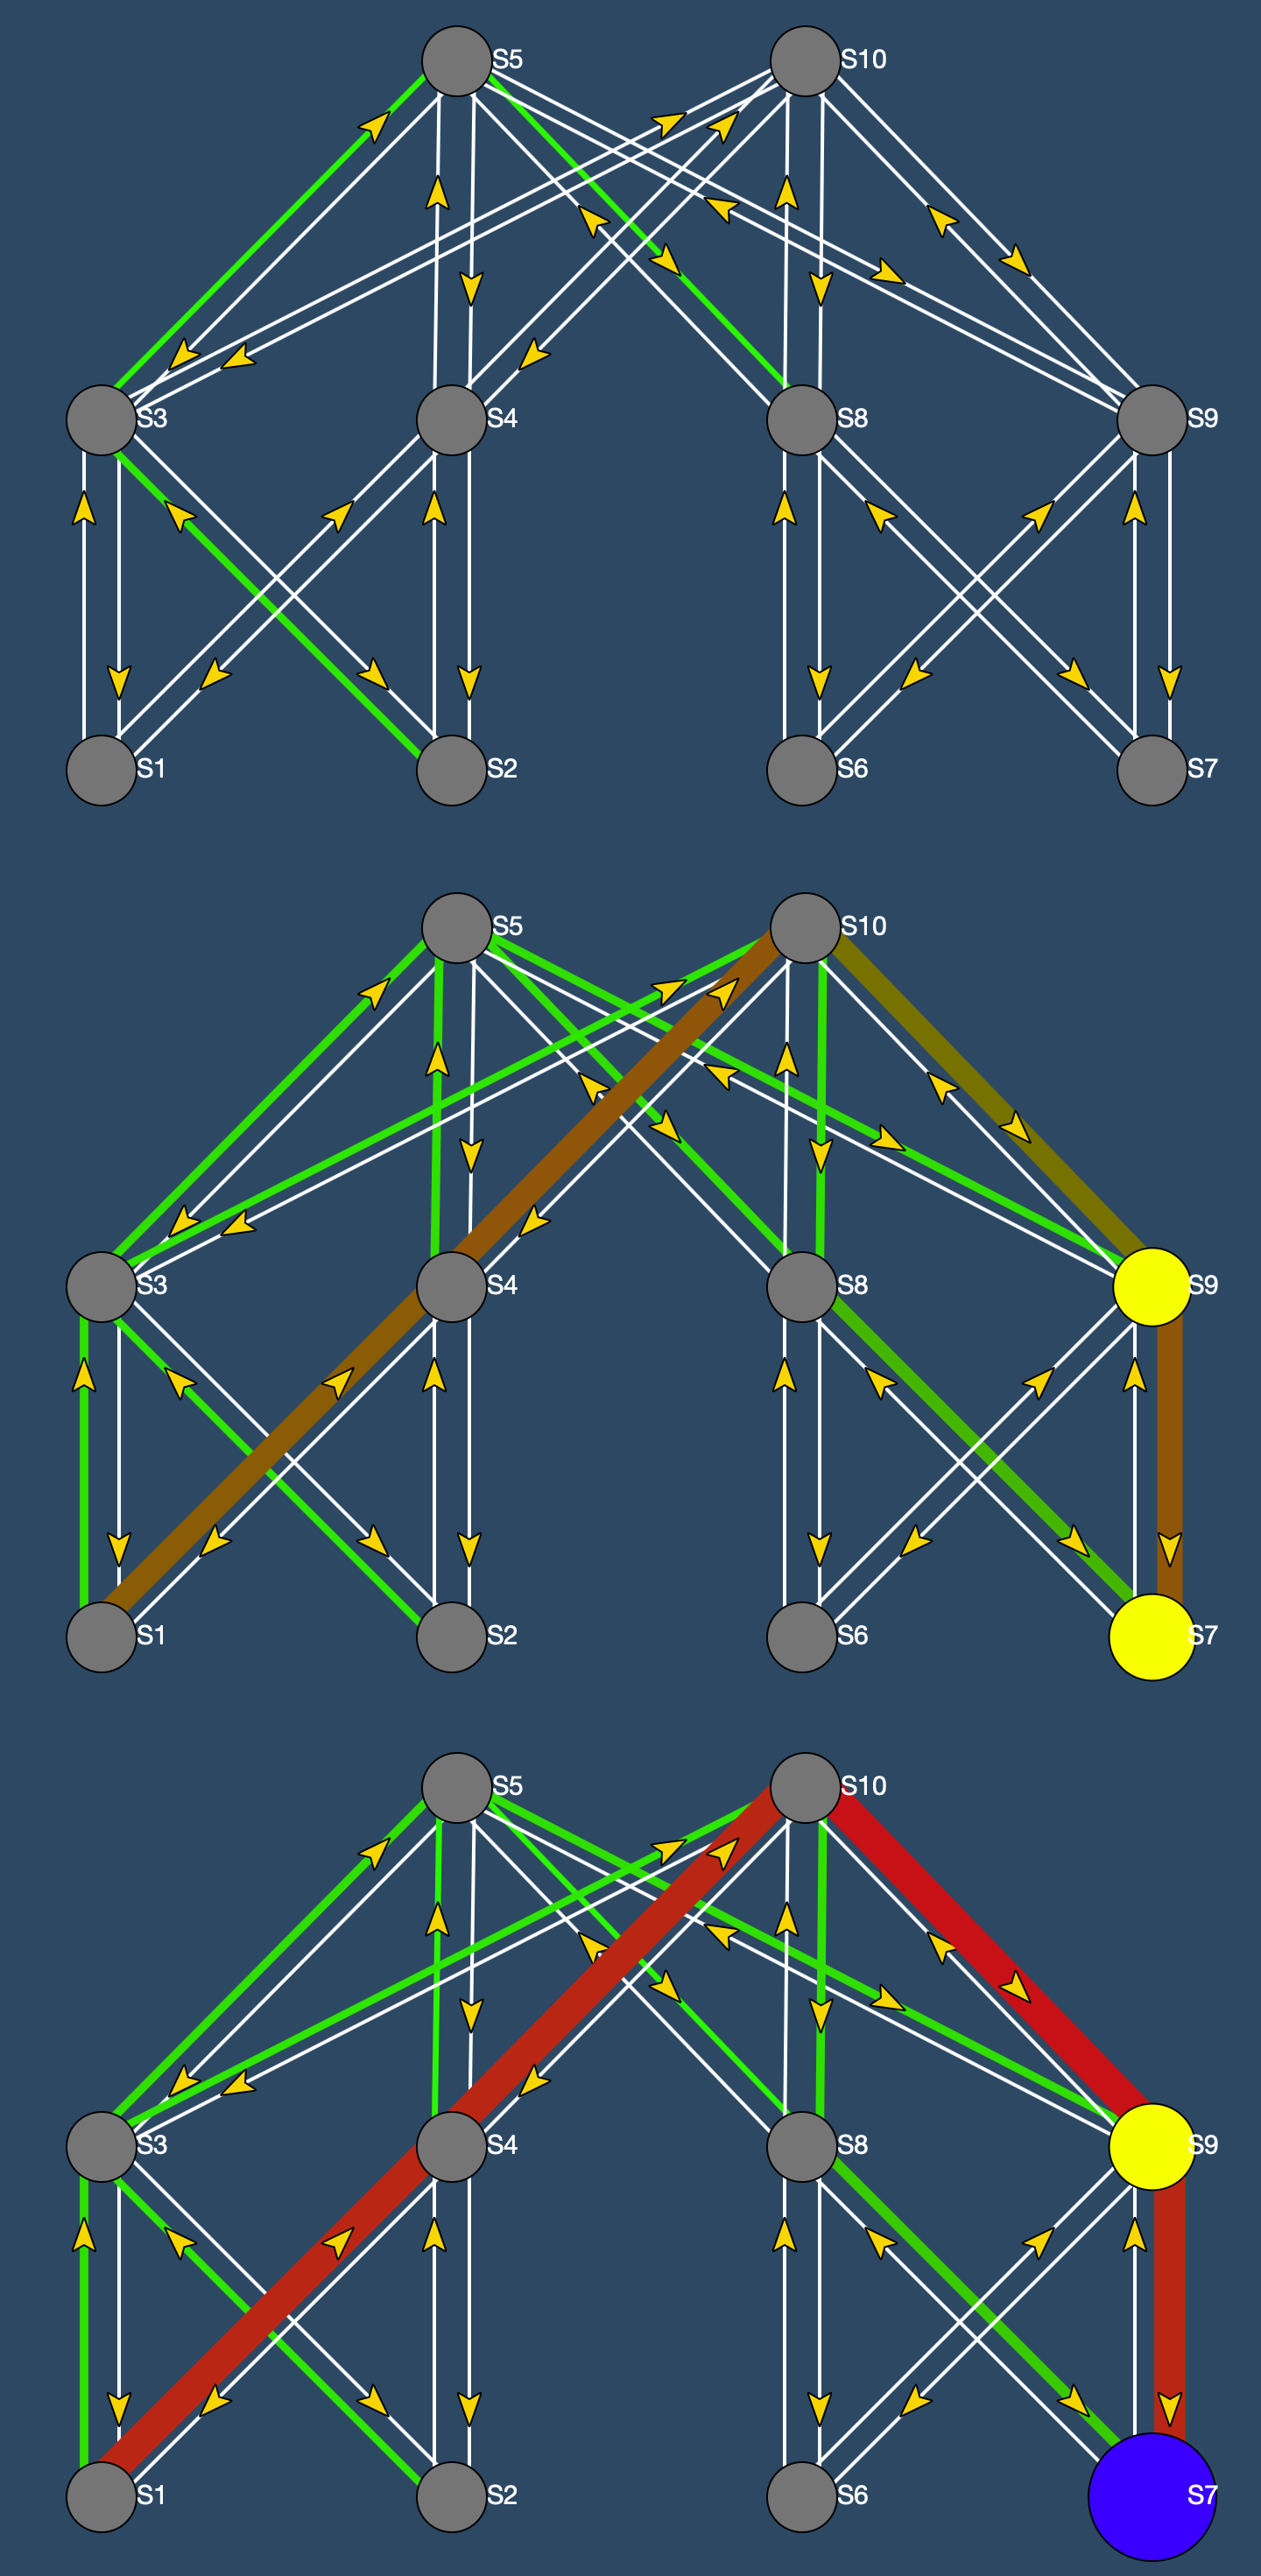
\includegraphics[width=20cm,height=25cm,keepaspectratio]{Figures/genview_async.png}
		\rule{35em}{0.5pt}
	\caption[Birds eye view, Asynchronous Incast]{Birds eye view of network at chronological points in time.}
	\label{fig:genview_async}
\end{figure}


\section{Link Underprovisioning}
\subsection{Description}
A link underprovision occurs when the link is operating at near, or maximum capacity for prolonged periods of time (of the order of milliseconds or seconds).
This usually requires the operator to provide additional bandwidth for the link.
It also leads to large buildup of queues in switches for prolonged periods of time.
\subsection{Configuration}
For creating a link underprovision scenario in our topology, we generate traffic of 6 Gbps from H3, H4, H5 and 1 Gbps from H1 and H2. The flow are routed
according to Figure \ref{fig:Synch Incast Topo} and get aggregated at switch 7.
\subsection{Diagnosis}
As stated before, a link will be underprovisioned if it is overutilized for a duration of the order of milliseconds.
If we find that the width of the peak as found in Algorithm 1 is of the order of milliseconds, and that the link is being overutilized, say by setting a threshold
to be average utilization greater than 0.8 * max capacity, then we classify the link to be overutilized.
\subsection{Results and Illustrations}
The above heuristic was applied to 2 different scenarios of link underprovision of varied transmission rates.
The resultant values of peak width calculated are given in table \ref{tab:Peak_Width}
\begin{table}[h]
\begin{center}
\begin{tabular}{ |p{3cm}|p{5cm}|  }
	\hline
	\multicolumn{2}{|c|}{Peak Width} \\
	\hline
	Scenario & Duration (in microseconds) \\
	\hline
	1 & 2575.626 \\
	2 & 4713.071 \\
	\hline
   \end{tabular}
\end{center}

\caption{Peak Width Duration for different scenarios of Link Underprovisioning}
% Help
\label{tab:Peak_Width}
\end{table}

The operator first looks at the recommendation given by the application as to what the fault is (Fig. \ref{fig:home_under}).
The operator looks at the birds eye view of the network and seens that there is massive buildup of queues along with maximum
capacity utilization of links.(Fig. \ref{fig:genview_under}).
Further, to help the network operator visualize the scenario, plots of ingress throughput and compositon of queue depth at 
trigger switch are plotted as shown in figure \ref{fig:ing_throughput_under}.
Looking at the plot of ingress throughput, the operator sees that there is one heavyhitter flow existing in the network.
He also looks at the composition of the queue depth to see that a large number of packets at the peak belong to this one flow and
that the queue only starts to buildup once this flow starts entering the switch.

These hints suggest a case of underprovisioned network.

\begin{figure}[htbp]
	\centering
		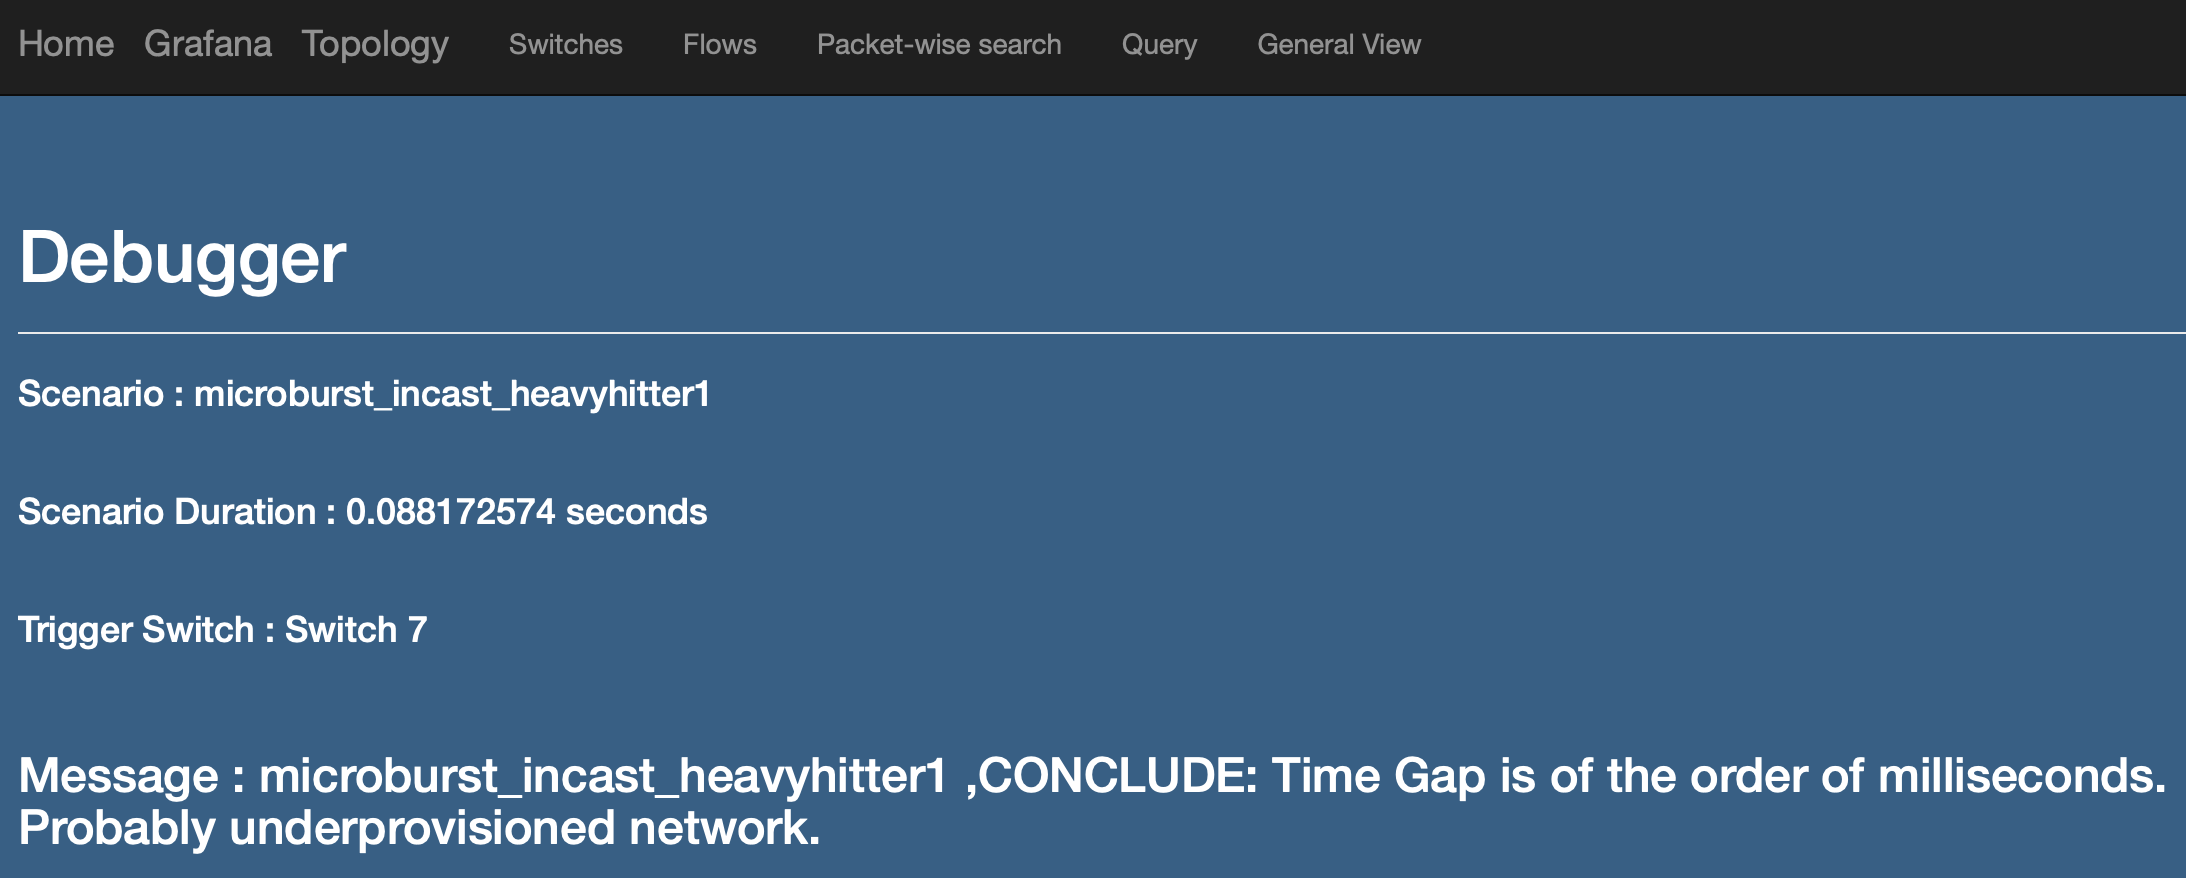
\includegraphics[width=1.0\columnwidth]{Figures/jindex_under.png}
		\rule{35em}{0.5pt}
	\caption[Debugger Home Page, Link Underprovisioning]{Message given to administrator}
	\label{fig:home_under}
\end{figure}
\begin{figure}[htbp]
	\centering
		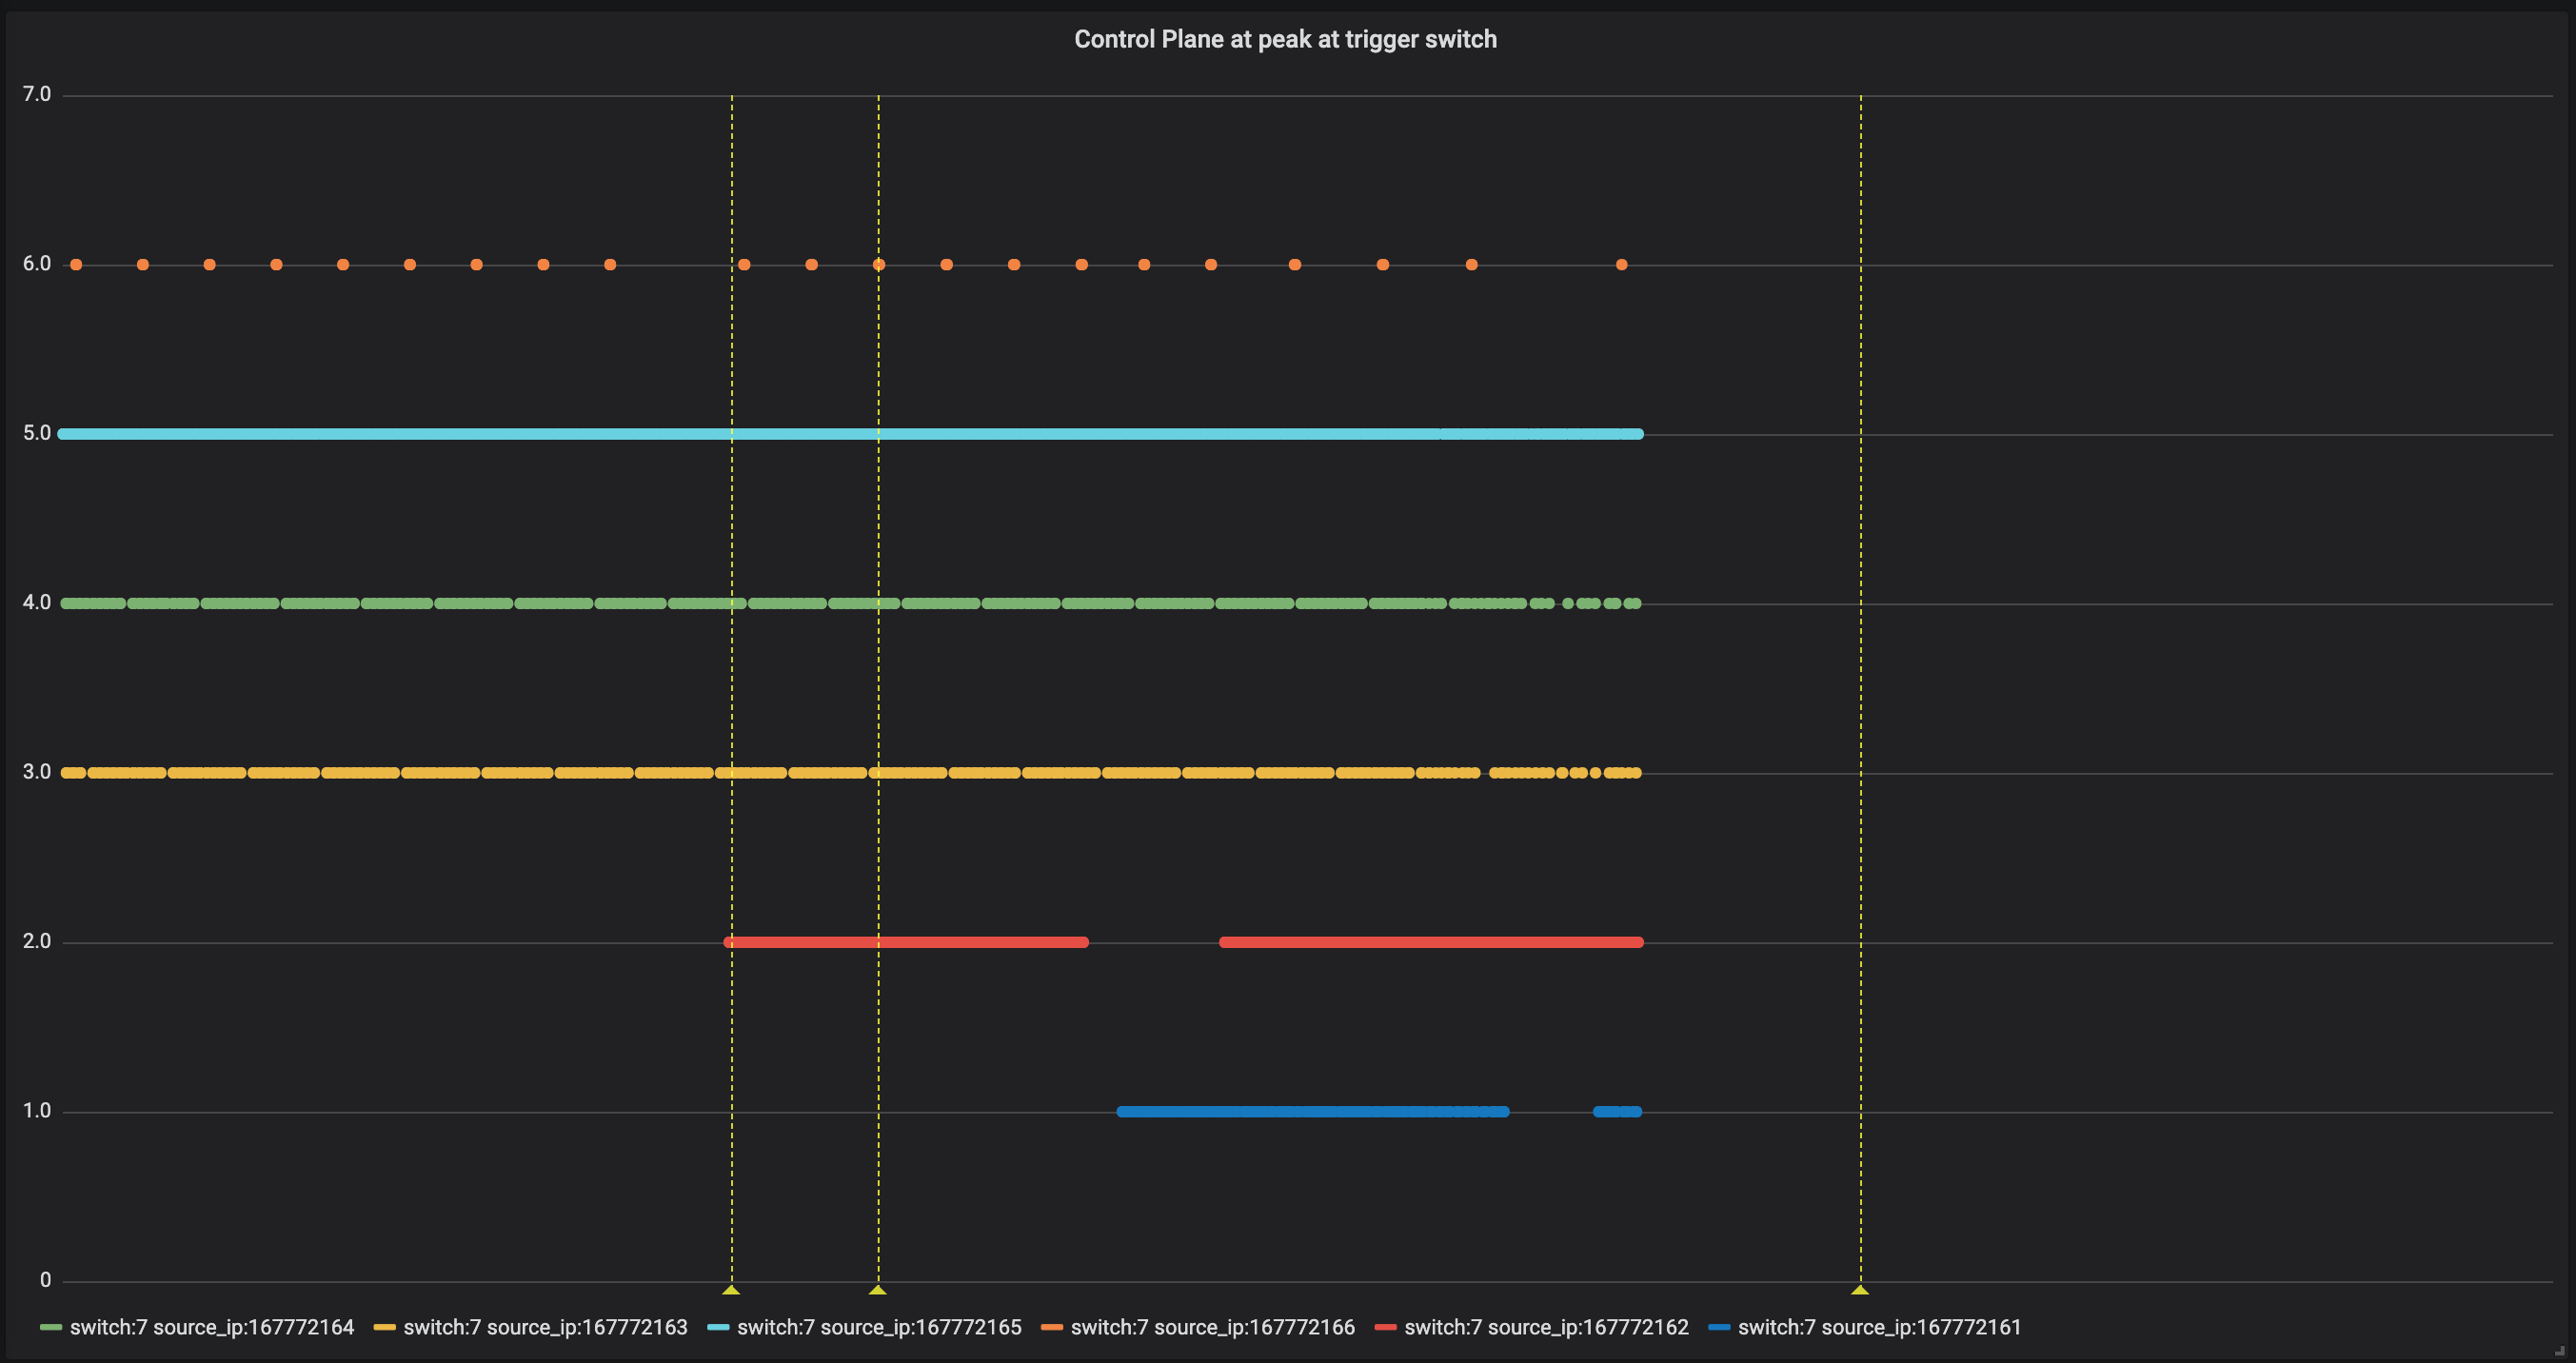
\includegraphics[width=1.0\columnwidth]{Figures/distribution_under.png}
		\rule{35em}{0.5pt}
	\caption[Packet Distribution at Trigger Switch, Link Underprovisioning]{Packet Distribution at Trigger Switch, Link Underprovisioning. Note the overlapping dots, showing link to be overutilized.}
	\label{fig:distribution_under}
\end{figure}
\begin{figure}[htbp]
	\centering
		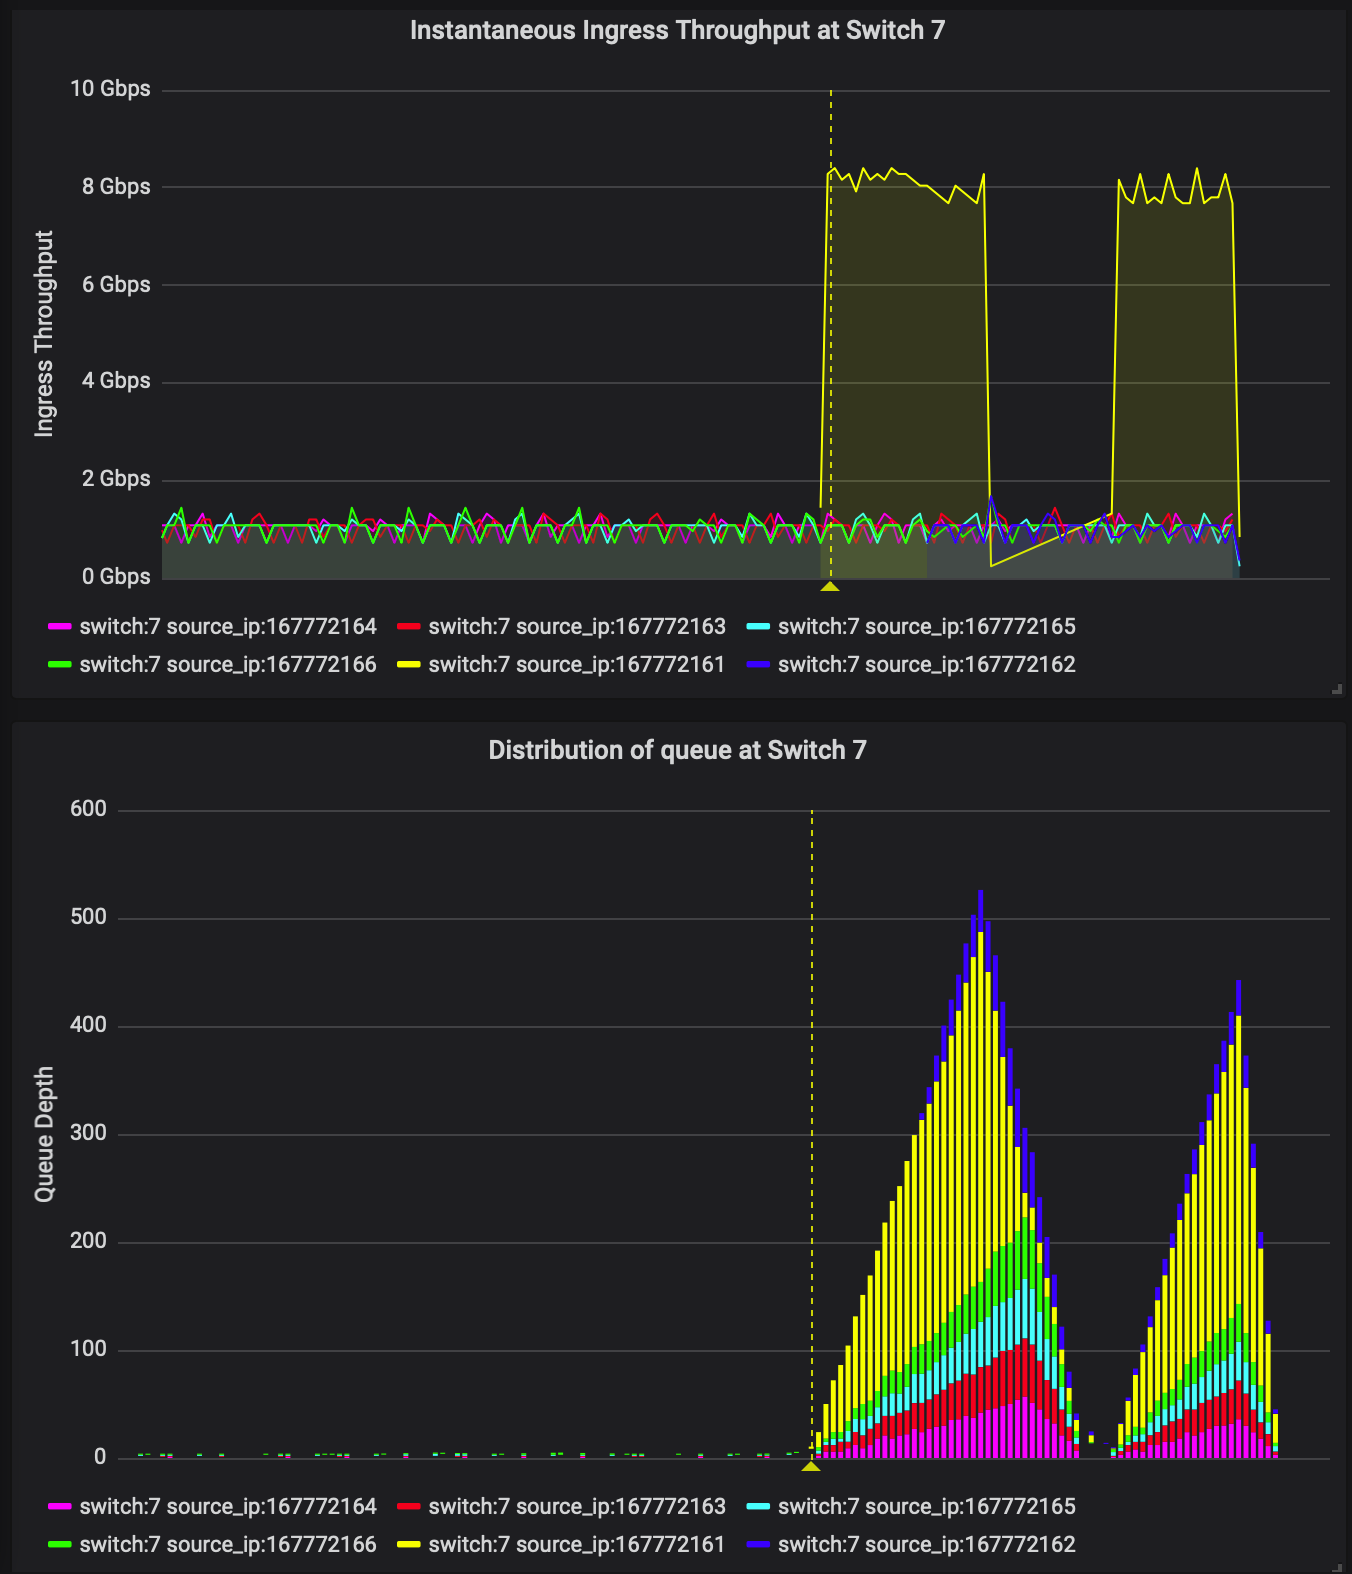
\includegraphics[width=1.0\columnwidth]{Figures/ingress_throughput_queue_comp_under.png}
		\rule{35em}{0.5pt}
	\caption[Ingress Throughput, Queue Composition at Trigger Switch, Link Underprovisioning]{Ingress Throughput, Queue Composition at Trigger Switch, Link Underprovisioning}
	\label{fig:ing_throughput_under}
\end{figure}


\begin{figure}[htbp]
	\centering
		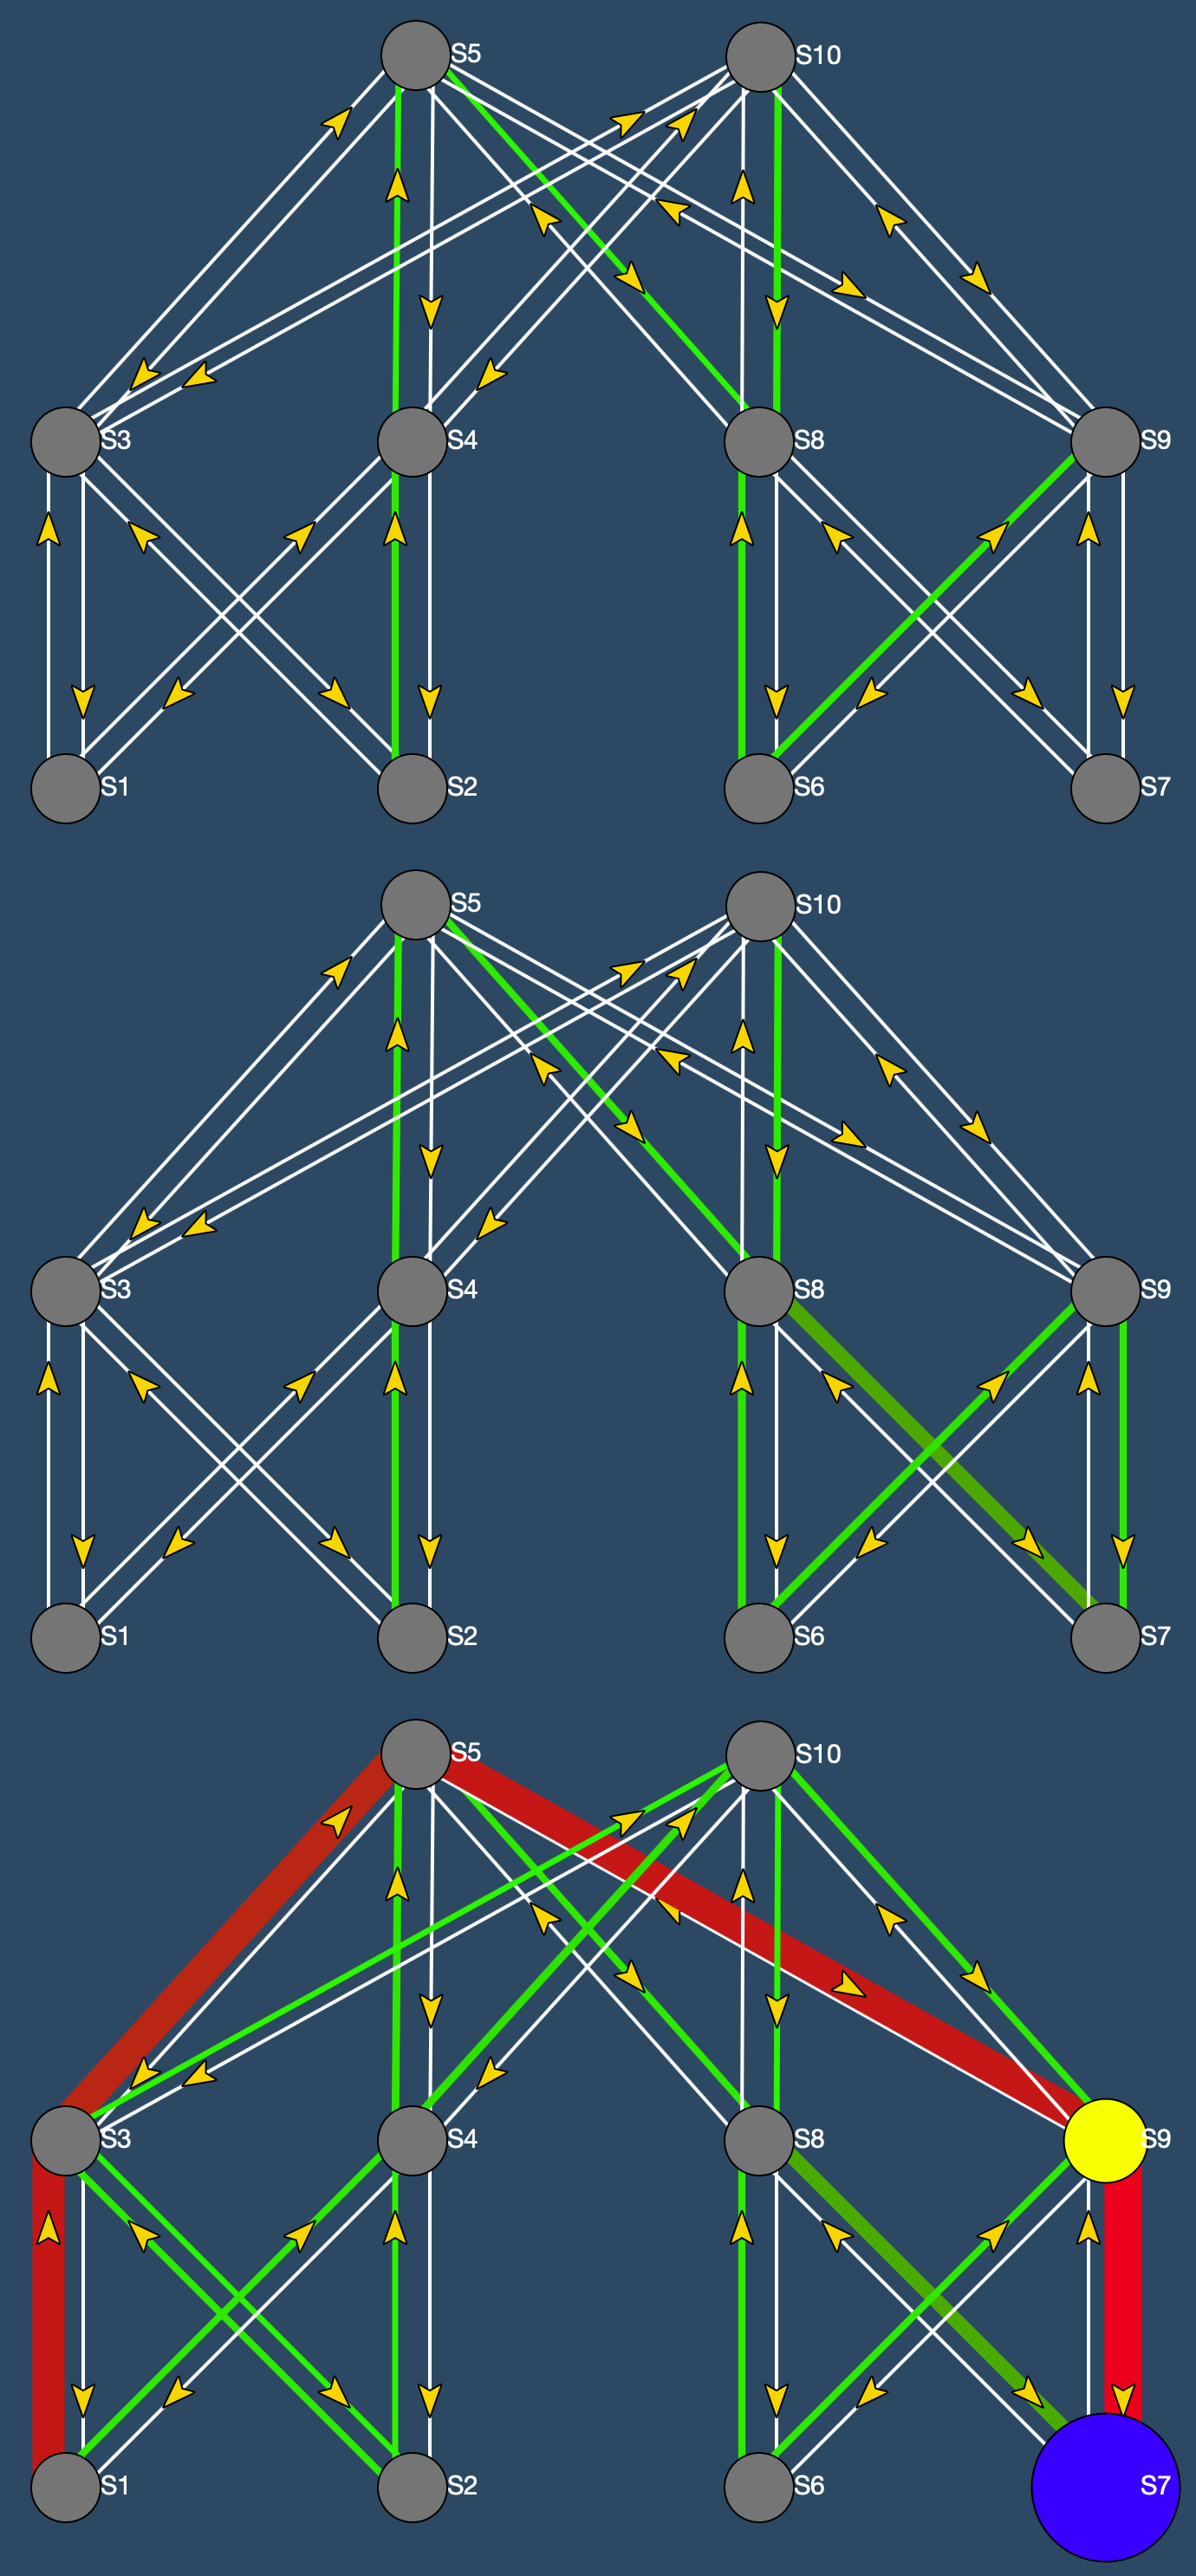
\includegraphics[width=20cm,height=25cm,keepaspectratio]{Figures/genview_under.png}
		\rule{35em}{0.5pt}
	\caption[Birds eye view, Link Underprovisioning]{Birds eye view of network at chronological points in time.}
	\label{fig:genview_under}
\end{figure}

\section{A unified scheme}

Based on the reasoning done in the preceding sections, a unified scheme to classify arbitrary scenarios based on the above discussion would be as follows:
\begin{itemize}
	\item Estimate the peak width in the graph
	\item If it is more than 1 millisecond, check if link is being overutilized. If so, it is probably a case of link underprovisioning.
	\item If it is less than 1 microsecond, calculate Jain's Fairness Index of packet distribution. If it is greater than 0.7, it is probably a synchronized incast. 
	\item Else, if it is less than 0.45, it is probably an asynchronous incast with heavy hitters present.
	\item Else (it is between 0.45 and 0.7), plot appropriate graphs for queue depth and link utilization and let the network operator deduce the exact problem.
\end{itemize}

In this way, we can isolate many such problems (for example,link failure 
and change of control plane policy), diagnose them on an individual basis using the relational model,
and at the end consolidate everything together into a single unified logic for diagnosing varied faults in a network.

Thus, this chapter and the previous chaper prove that the relational model is an effective means for debugging
the network and identifying issues. This, coupled with effective tools and visualizations built in this thesis
demonstratethat large insights can be gained into network functioning.

